\documentclass[twocolumn]{svjour3}          % twocolumn
%
\smartqed  % flush right qed marks, e.g. at end of proof
%
\usepackage{graphicx}
\usepackage{pst-node}
\usepackage{pst-rel-points}
\usepackage{url}
\usepackage{setspace}
\usepackage{listings}
\usepackage{natbib}

\usepackage{ulem}
\usepackage{multirow}
\usepackage{xcolor,colortbl}

% \usepackage{mathptmx}      % use Times fonts if available on your TeX system
%
\lstset{language=C,basicstyle=\footnotesize\ttfamily ,columns=fullflexible,keywordstyle=,morekeywords=}

\journalname{Innovations in Systems and Software Engineering}
%
%%%%%%%%%%%%%%%%%%%%%%%%%%%%%%%%%%%%%%%%
%%%%%%% New Commands %%%%%%%%%%%%%%%%%%
%%%%%%%%%%%%%%%%%%%%%%%%%%%%%%%%%%%%%%%%
\newcommand{\cmt}[1]{} % commented out stuff
\newcommand{\is}{\itemsep -1mm} % reduce space between items
\newcommand{\hide}[1]{} % hidden for double blind review

\newcommand{\p}{\ensuremath{p}}
\newcommand{\q}{\ensuremath{q}}
\newcommand{\s}{\ensuremath{s}}
\newcommand{\f}{\ensuremath{f}}
\newcommand{\myr}{\ensuremath{r}}
\newcommand{\I}{\ensuremath{I}}
\newcommand{\x}{\ensuremath{x}}

\newcommand{\Left}{\ensuremath{Left}}
\newcommand{\Right}{\ensuremath{Right}}
\newcommand{\Parent}{\ensuremath{Parent}}  


\newcommand{\B}{\mbox{\tt B}}
\renewcommand{\a}{\mbox{\tt a}}
\renewcommand{\b}{\mbox{\tt b}}
\renewcommand{\c}{\mbox{\tt c}}
\renewcommand{\d}{\mbox{\tt d}}
\newcommand{\m}{\mbox{\tt m}}

\newcommand{\alias}[1]{\ensuremath{{#1}^{\dag}}}
\newcommand{\aliasinfo}[1]{\ensuremath{\{\myr | \myr = #1 \vee \epsilon \in D_F^{\din}[\myr,#1] \vee \epsilon \in D_F^{\din}[#1, \myr] \}}}
\newcommand{\drct}{\ensuremath{D}}
\newcommand{\indrct}{\ensuremath{I}}
\newcommand{\heap}{\ensuremath{\mathcal{H}}}
\newcommand{\fields}{\ensuremath{\mathcal{F}}}
\newcommand{\upath}{\ensuremath{\mathcal{U}}}
\newcommand{\shape}{\mbox{shape}}
\newcommand{\nat}{\ensuremath{\mathcal{N}}}

\newcommand{\mwedge}{\; \wedge \;}
\newcommand{\mvee}{\; \vee \;}
\newcommand{\mcup}{\; \cup \;}
\newcommand{\mjoin}{\; \Join \;}
\newcommand{\mbackslash}{\; \backslash \;}
\newcommand{\subC}{\mbox{\scalebox{0.6}{\Cycle}}}
\newcommand{\subD}{\mbox{\scalebox{0.6}{\Dag}}}

\newcommand{\epsilonset}{\ensuremath{\{\epsilon\}}}
\newcommand{\epsilonpairset}{\ensuremath{\{\epsilon,\epsilon\}}}

\newcommand{\dout}{\mbox{\footnotesize out}}
\newcommand{\din}{\mbox{\footnotesize in}}
\newcommand{\dkill}{\mbox{\footnotesize kill}}
\newcommand{\dgen}{\mbox{\footnotesize gen}}

\newcommand{\GenC}[1]{\ensuremath{{#1}_{\subC}^{\dgen}}}
\newcommand{\GenD}[1]{\ensuremath{{#1}_{\subD}^{\dgen}}}
\newcommand{\KillC}[1]{\ensuremath{{#1}_{\subC}^{\dkill}}}
\newcommand{\KillD}[1]{\ensuremath{{#1}_{\subD}^{\dkill}}}
\newcommand{\InC}[1]{\ensuremath{{#1}_{\subC}^{\din}}}
\newcommand{\InD}[1]{\ensuremath{{#1}_{\subD}^{\din}}}
\newcommand{\OutC}[1]{\ensuremath{{#1}_{\subC}^{\dout}}}
\newcommand{\OutD}[1]{\ensuremath{{#1}_{\subD}^{\dout}}}

\newcommand{\merge}{\ensuremath{\mathrm{merge}}}
\newcommand{\project}[2]{\ensuremath{#1\triangleright\!\!#2}}
\newcommand{\num}[1]{\ensuremath{|#1|}}
\newcommand{\remOne}[2]{\ensuremath{#1 \ominus #2}}
\newcommand{\remAll}[2]{\ensuremath{#1\uminus #2}}

\newcommand{\Gen}[1]{{\mbox{{\tt gen}}_{\mbox{\scalebox{0.6}{{\tt #1}}}}}}
\newcommand{\Kill}[1]{{\mbox{{\tt kill}}_{\mbox{\scalebox{0.6}{{\tt #1}}}}}}
\newcommand{\mb}[1]{\mbox{{\tt #1}}}
\newcommand{\DFM}[2]{\ensuremath{P_F[#1,#2]}}
\newcommand{\IFM}[2]{\ensuremath{I_F[#1,#2]}}
\newcommand{\Tree}{{\tt Tree}}
\newcommand{\Dag}{{\tt Dag}}
\newcommand{\Cycle}{{\tt Cycle}}
\newcommand{\upstmt}[1]{{\tt p$\rightarrow$f = #1}}
\newcommand{\TV}{{\tt TrueVars}}
\newcommand{\fieldD}[2]{\ensuremath{{#1}_{#2}^\drct}}
\newcommand{\fieldI}[3]{\ensuremath{{#1}_{#2}^{\indrct#3}}}
\newcommand{\range}[3]{\ensuremath{{#1} \leq {#2} \leq {#3}}}
\newcommand{\U}{{\rm Unknown}}
\newcommand{\fig}[1]{\includegraphics[scale=.5]{#1}}
\newcommand{\false}{\textbf{False}}
\newcommand{\true}{\textbf{True}}

\begin{document}

\title{Precise Shape Analysis using Field Sensitivity%\thanks{Grants or other notes
%about the article that should go on the front page should be
%placed here. General acknowledgments should be placed at the end of the article.}
}
%\subtitle{Do you have a subtitle?\\ If so, write it here}

%\titlerunning{Short form of title}        % if too long for running head

\author{Sandeep Dasgupta         	\and
        Amey Karkare  				\and
		Vinay Kr Reddy  
}

%\authorrunning{Short form of author list} % if too long for running head

\institute{Sandeep Dasgupta \at
	Intel Technology India Pvt. Ltd. \\
		%              Tel.: +123-45-678910\\
		%              Fax: +123-45-678910\\
		%              \email{fauthor@example.com}           %  \\
			%             \emph{Present address:} of F. Author  %  if needed
           \and
           Amey Karkare \at
              		Department of Computer Science and Engineering,\\
 				 	Indian Institute of Technology Kanpur, Kanpur, India\\
			\and		
		   Vinay Kr Reddy \at
              		Department of Computer Science and Engineering,\\
 				 	Indian Institute of Technology Kanpur, Kanpur, India\\
}

\date{Received: date / Accepted: date}
% The correct dates will be entered by the editor


\maketitle

\begin{abstract}
\documentclass[12pt,twoside,openright]{report}
\usepackage[T1]{fontenc}
\usepackage{amssymb}
\usepackage{graphicx}
\usepackage{latexsym}
\usepackage{amsmath}
\usepackage{array}
\usepackage{amsthm}
\usepackage{wrapfig}
\usepackage{geometry}
\usepackage{pstricks}
\usepackage{pst-node,pst-tree}
\usepackage{pst-rel-points}
\usepackage{flexiprogram}
\geometry{verbose,a4paper,tmargin=15mm,bmargin=30mm,lmargin=30mm,rmargin=20mm}
\usepackage{graphics}
\usepackage{setspace}
\usepackage{framed}
\usepackage{verbatim}
\usepackage{epsfig}
\usepackage{fancyheadings}
\usepackage{multirow}
\setcounter{secnumdepth}{5}
\setcounter{tocdepth}{5}
\onehalfspacing
\makeatletter
\setlength{\headheight}{10pt}
\pagestyle{fancyplain}
\renewcommand{\chaptermark}[1]{\markboth{#1}{}}
\lhead{\fancyplain{}{\thepage}}
\chead{}
\rhead{\fancyplain{}{\textit{\leftmark}}}
\lfoot{}
\cfoot{}
\rfoot{}
\linespread{1.3}


%%%%%%%%%%%%%%%%%%%%%%%%%%%%%%%%%%%%%%%%
%%%%%%% theorems and definitions %%%%%%%
%%%%%%%%%%%%%%%%%%%%%%%%%%%%%%%%%%%%%%%%
\newtheorem{definition}{Definition}[chapter]
\newtheorem{example}{Example}[chapter]
%%%%%%%%%%%%%%%%%%%%%%%%%%%%%%%%%%%%%%%%
%%%%%%% New Commands %%%%%%%%%%%%%%%%%%
%%%%%%%%%%%%%%%%%%%%%%%%%%%%%%%%%%%%%%%%
\newcommand{\cmt}[1]{} 
\newcommand{\p}{\ensuremath{p}}
\newcommand{\q}{\ensuremath{q}}
\newcommand{\s}{\ensuremath{s}}
\newcommand{\myr}{\ensuremath{r}}

\newcommand{\B}{\mbox{\tt B}}
\renewcommand{\a}{\mbox{\tt a}}
\renewcommand{\b}{\mbox{\tt b}}
\renewcommand{\c}{\mbox{\tt c}}
\renewcommand{\d}{\mbox{\tt d}}
\newcommand{\m}{\mbox{\tt m}}

\newcommand{\drct}{\ensuremath{D}}
\newcommand{\indrct}{\ensuremath{I}}
\newcommand{\heap}{\ensuremath{\mathcal{H}}}
\newcommand{\fields}{\ensuremath{\mathcal{F}}}
\newcommand{\upath}{\ensuremath{\mathcal{U}}}
\newcommand{\shape}{\mbox{shape}}
%\newcommand{\nat}{\ensuremath{\bbbn}}
\newcommand{\nat}{\ensuremath{\mathcal{N}}}

\newcommand{\mwedge}{\  \wedge \ }
\newcommand{\mvee}{\  \vee \ }
\newcommand{\mcup}{\  \cup \ }
\newcommand{\mjoin}{\  \Join \ }
\newcommand{\mbackslash}{\  \backslash \ }
\newcommand{\subC}{\mbox{\scalebox{0.6}{\Cycle}}}
\newcommand{\subD}{\mbox{\scalebox{0.6}{\Dag}}}

\newcommand{\epsilonset}{\ensuremath{\{\epsilon\}}}
\newcommand{\epsilonpairset}{\ensuremath{\{\epsilon,\epsilon\}}}

\newcommand{\dout}{\mbox{\footnotesize\em out}}
\newcommand{\din}{\mbox{\footnotesize\em in}}
\newcommand{\dkill}{\mbox{\footnotesize\em kill}}
\newcommand{\dgen}{\mbox{\footnotesize\em gen}}

\newcommand{\GenC}[1]{\ensuremath{{#1}_{\subC}^{\dgen}}}
\newcommand{\GenD}[1]{\ensuremath{{#1}_{\subD}^{\dgen}}}
\newcommand{\KillC}[1]{\ensuremath{{#1}_{\subC}^{\dkill}}}
\newcommand{\KillD}[1]{\ensuremath{{#1}_{\subD}^{\dkill}}}
\newcommand{\InC}[1]{\ensuremath{{#1}_{\subC}^{\din}}}
\newcommand{\InD}[1]{\ensuremath{{#1}_{\subD}^{\din}}}
\newcommand{\OutC}[1]{\ensuremath{{#1}_{\subC}^{\dout}}}
\newcommand{\OutD}[1]{\ensuremath{{#1}_{\subD}^{\dout}}}

\newcommand{\merge}{\ensuremath{\mathrm{merge}}}
\newcommand{\project}[2]{\ensuremath{#1\triangleright\!\!#2}}
\newcommand{\num}[1]{\ensuremath{|#1|}}
\newcommand{\first}[1]{\ensuremath{#1. \mathrm{fst}}}
\newcommand{\second}[1]{\ensuremath{#1. \mathrm{snd}}}

\newcommand{\remOne}[2]{\ensuremath{#1 \ominus #2}}

\newcommand{\Gen}[1]{{\mbox{{\tt gen}}_{\mbox{\scalebox{0.6}{{\tt #1}}}}}}
\newcommand{\Kill}[1]{{\mbox{{\tt kill}}_{\mbox{\scalebox{0.6}{{\tt #1}}}}}}
\newcommand{\mb}[1]{\mbox{{\tt #1}}}
\newcommand{\DFM}[2]{\ensuremath{D_F[#1,#2]}}
\newcommand{\IFM}[2]{\ensuremath{I_F[#1,#2]}}
\newcommand{\Tree}{{\tt Tree}}
\newcommand{\Dag}{{\tt Dag}}
\newcommand{\Cycle}{{\tt Cycle}}
\newcommand{\upstmt}[1]{{\tt p$\rightarrow$f = #1}}
\newcommand{\TV}{{\tt TrueVars}}
\newcommand{\fieldD}[2]{\ensuremath{{#1}_{#2}^\drct}}
\newcommand{\fieldI}[3]{\ensuremath{{#1}_{#2}^{\indrct#3}}}
\newcommand{\range}[3]{\ensuremath{{#1} \leq {#2} \leq {#3}}}
\newcommand{\fig}[1]{\includegraphics[scale=.5]{#1}}
\newcommand{\false}{\textbf{False}}
\newcommand{\true}{\textbf{True}}
\newcommand{\anysup}{\ensuremath{\ast}}
\makeatother
\renewcommand\bibname{References}

\begin{document}
%
%\thispagestyle{empty}
%%\chapter*{Declaration}
\vspace*{5cm}
\begin{center}
\underline{\textbf{Declaration}}
\end{center}

I declare that this written submission represents my ideas in my own 
words except Appendix A and B whose contents are borrowed from Ghiya et. al.~\cite{Ghiya96} and Marron et. al.~\cite{marron06static} respectively for the 
ease of reference. The places where others' ideas or words have been included, I have adequately cited and 
referenced the original sources.
\newpage

%
\input{abstract_matter.tex} 

\end{document}



%
%\keywords{First keyword \and Second keyword \and More}
\keywords{Shape analysis \and dataflow analysi \and pointer analysis \and static analysis \and heap analysis}
\end{abstract}

%%%%%%%%%%%%%%%%%%%%%%%%%%%%%%%%%%%%%%%%%%%%%%%%%%%%%
\section{Introduction}
%%%%%%%%%%%%%%%%%%%%%%%%%%%%%%%%%%%%%%%%%%%%%%%%%%%%%
Hardware  and Software  revolutions  in past  few years  have
brought in  two significant challenges:  (a) High performance
computing  is now  accessible  to end  users (scientists  and
engineers) in the forms of multi-core and GPU processors at a
very  low cost.   However, these  end users,  who  are domain
experts,  find  it difficult  to  acquire  expertise to  take
advantage of  the compute power available  at their disposal.
As a result, the compute remains significantly underutilized.
The  tasks  of  helping  programmers ``think  parallel''  and
providing   them  with   working  parallel   environment  are
considered   the  top   challenges   in  parallel   computing
research~\cite{top10,  wrinn08parallel}.   (b)  The  cost  of
failure of software is increasing with the growing complexity
of software. The cost of software failure was estimated to be
USD   6.18  Trillion   in  the   year  2009~\cite{roger09it}.
Therefore, it  is becoming more and more  important to verify
the correctness of a  software program before its deployment.
The complexity of hardware  and software systems require that
the solutions  to the above challenges have  to be automated.
We  need  parallelizing   compilers  that  can  automatically
convert  sequential programs to  parallel one,  and verifying
compilers that can prove the correctness of programs.

Programs  in  all   modern  programming  languages  use  heap
intensively.  Any  non  trivial  analysis of  these  programs
requires  precise reasoning  about the  heap  structures. The
reasoning  is complex  because  the heap  structures are  not
static but  are manipulated dynamically  during the execution
of the  program.  {\em  Shape analysis} is  the term  for the
class of  static analysis techniques  that are used  to infer
useful  properties  about heap  structures  and the  programs
manipulating  the heap.   The shape  information of  the heap
data structures  can be used by variety  of applications, for
e.g.    compile  time  optimizations,   compile-time  garbage
collection,  debugging, verification,  instruction scheduling
and parallelization.

In the  last two  decades, several shape  analysis techniques
have  been  proposed  in  literature.  However,  there  is  a
trade-off between  speed and precision  for these techniques,
thus  making them  suitable  either for  verification or  for
optimization,   but  not   both.    Precise  shape   analysis
algorithms~\cite{Sagiv96,shaham03heap,distefano06local,hackett05region}
are not  practical for an optimizing compilers  as they scale
poorly to  the large heap manipulating  programs.  To achieve
scalability,  the  optimizing  compilers use  shape  analysis
algorithms~\cite{Chase90,Ghiya96,marron06static}  that  trade
precision for  speed by  ignoring certain properties  of heap
structures  (for example,  the calling  context or  the field
connectivity between the pointers).

In  this  paper,  we   present  a  field  sensitive,  context
sensitive shape analysis technique that uses field-based path
information  to  infer the  shapes  of  heap structures.  The
novelty  of  our  approach  lies  in the  way  we  use  field
information to remember the paths that result in a particular
shape  (Tree,  DAG,  Cycle).   This  allows  us  to  identify
transitions from a conservative shape to a more precise shape
(i.e., from Cycle to DAG, from  Cycle to Tree and from DAG to
Tree) due to destructive updates.  This in turn enables us to
infer precise shape information.

Our analysis captures the field sensitivity information using
two components: (a) Field based boolean variables to remember
the direct connections between two pointer variables, and (b)
Path  matrices  that  store  the  approximate  paths  between
pointer  variables.  The  shape of  a pointer  variable  at a
given program point is inferred from these two components.

This paper makes the following contributions:
\begin{enumerate}
\item We present a novel field based shape analysis technique
  that uses  limited path information to  infer precisely the
  shapes of  heap structures. We  propose the analysis  as an
  instance  of a  forward data  flow analysis  framework, and
  describe in details the components of the framework.
\item We describe a flow sensitive, context sensitive
  implementation of our analysis as a plug-in for GCC version
  4.5.0~\cite{gcc-web}. we present experimental evaluation
  and comparison of our analysis with an existing field
  insensitive approach~\cite{Ghiya96} on several benchmark
  programs. 
\item  We propose some  enhancements to  our analysis:  (a) A
  {\em Field-subset} based analysis to improve precision when
  auxiliary  fields\footnote{Fields that  are  used only  for
    diagnostic   or  debugging  purpose,   or  unused   by  a
    significant part  of the  program.}  are present  in data
  structures, and (b)  shape-based context sensitive analysis
  to improve  memory footprint and  speed when the  number of
  contexts is huge.
\end{enumerate}

The paper is organized as follows: 
We demonstrate the working of our analysis using a motivating
example  in Section~\ref{sec:motiv}, and  explain intuitively
the key concepts.
%%
Section~\ref{sec:Formal_Definitions}  presents  the notations
and     definitions    used     by    our     analysis    and
Section~\ref{sec:Analysis} describes the details of the
analysis.
%%
%Section~\ref{subsec:Interprocedural_Analysis}    describes   the
%call-strings   approach  we   used  to   incorporate  context
%sensitivity in the analysis.
%%
%The   properties   of   our   analysis   are   described   in
%Section~\ref{subsec:props}.
%%
Section~\ref{sec:implementation_results}     describes    the
baseline      approach      (field     insensitive      shape
analysis~\cite{Ghiya96}),  the  benchmark  programs  and  our
experimental evaluation.
%%
Section~\ref{sec:Enhancements} describes some enhancements
over our current scheme. 
%%
We discuss some of the prior works on shape analysis in
Section~\ref{sec:bgrel}. 
%% 
Section~\ref{sec:concl} concludes the
paper and gives directions for future work.


We start  out with  motivating examples that  also illustrate
the workings of our analysis.


%%%%%%%%%%%%%%%%%%%%%%%%%%%%%%%%%%%%%%%%%%%%%%%%%%%%%
\section{A Motivating Example}\label{sec:motiv}
%%%%%%%%%%%%%%%%%%%%%%%%%%%%%%%%%%%%%%%%%%%%%%%%%%%%%
Following the
literature~\cite{Ghiya96,Sagiv96,marron06static},
we define the shape attribute for a pointer $\p$
as:
\begin{eqnarray*}
  \p.\shape = \left\{ \begin{array}{@{}rl@{}}
    \Cycle & \mbox{If a cycle can be reached from $\p$} \\ 
    \Dag & \mbox{Else if a DAG can be reached from $\p$} \\
    \Tree & \mbox{Otherwise} \\
  \end{array} \right.
\end{eqnarray*}
where the heap is visualized as a directed graph, and cycle
and DAG have there natural graph-theoretic meanings. For each
pointer variable, our analysis computes the shape attribute
of the data structure pointed to by the variable.  We use the
code fragment in Fig.~\ref{fig:motiv1} to motivate the need
for a field sensitive shape analysis.

\begin{figure}[t]
\begin{center}
  \scalebox{.99}{
    \begin{tabular}{c}
      {\small \tt
        \begin{tabular}[b]{rl}
          &int main() \{ \\
	  {\em \scriptsize S1:}& \quad tree root; \\
	  {\em \scriptsize S2:}& \quad \ldots        \\
          {\em \scriptsize S3:}& \quad mirror(root); \\
          {\em \scriptsize S4:}& \quad treeAdd(root); \\ 
          {\em \scriptsize S5:}& \quad \ldots \\ 
          &\} \\ \\
          & void mirror(tree t) \{ \\
          {\em \scriptsize S11:}& \quad tl  = t->left; \\
          {\em \scriptsize S12:}& \quad tr = t->right; \\
          {\em \scriptsize S13:}& \quad mirror(tl); \\
          {\em \scriptsize S14:}& \quad mirror(tr); \\
          {\em \scriptsize S15:}& \quad t->left  = tr; \\
          {\em \scriptsize S16:}& \quad t->right = tl; \\
          &\} \\ \\
	  & int treeAdd(tree t) \{     \\ 
	  {\em \scriptsize S21:}& \quad if (t == NULL)           \\ 
	  {\em \scriptsize S22:}& \quad \quad return 0;           \\ 
	  {\em \scriptsize S23:}& \quad tl = t$\rightarrow$left;    \\
          {\em \scriptsize S24:}& \quad treeAdd(tl); \\
          {\em \scriptsize S25:}& \quad tr = t$\rightarrow$right; \\
	  {\em \scriptsize S26:}& \quad treeAdd(tl); \\
	  {\em \scriptsize S27:}& \quad t$\rightarrow${num} = tl$\rightarrow${num} + tr$\rightarrow${num}; \\
	  &\}
        \end{tabular}
      } \\ \scalebox{0.80}{(a)} \\ \\ %\hline \\ \\
      {\small \tt
        \begin{tabular}[b]{l}
          typedef struct treenode tree;\\
          struct treenode \{ \\
            \quad int num; \\
            \quad tree *left; \\
            \quad tree *right; \\
            \};
        \end{tabular}
      } 
      \hskip -10mm\includegraphics[scale=
        .4]{Figures/tree_grph.eps} \\
      \scalebox{0.8}{(b)} \\ %\hline
    \end{tabular}}
\end{center}
\caption{\label{fig:motiv1} A motivating example. The program
  (a) manipulates  the heap structures created by using the
  basic data structure as shown in (b).}
\end{figure}


\begin{figure}[t]
\begin{center}
  {\small \tt 
    \begin{tabular}[b]{|l|@{}c@{}|} \hline
      {\rm Stmt} & {\rm Path matrix  $P_F$ after the stmt}  \\ \hline
      \multicolumn{2}{c}{} \\ \hline
      {\em \scriptsize S1} &
      \begin{tabular}{|p{3mm}||p{6mm}|p{12mm}|p{22mm}|} \hline
        &  t         & tl        & tr   \\ \hline\hline
  	t  	& $\emptyset$   & ${\tt \{\fieldD{\lft}{}\}}$    & $\emptyset$ \\ \hline
  	tl  & $\emptyset$   & $\emptyset$   & $\emptyset$   \\ \hline
  	tr  & $\emptyset$   & $\emptyset$   & $\emptyset$   \\ \hline
      \end{tabular} \\ \hline
      \multicolumn{2}{c}{} \\ \hline
      {\em \scriptsize S2} &				
      \begin{tabular}{|p{3mm}||p{6mm}|p{12mm}|p{22mm}|} \hline
        &  t         & tl        & tr   \\ \hline\hline
  	t  	& $\emptyset$   & ${\tt \{\fieldD{\lft}{}\}}$    & ${\tt \{\fieldD{\rht}{}\}}$ \\ \hline
  	tl  & $\emptyset$   & $\emptyset$   & $\emptyset$   \\ \hline
  	tr  & $\emptyset$   & $\emptyset$   & $\emptyset$   \\ \hline
      \end{tabular} \\ \hline
      \multicolumn{2}{c}{} \\ \hline
      {\em \scriptsize S5} &				
      \begin{tabular}{|p{3mm}||p{6mm}|p{12mm}|p{22mm}|} \hline
        &  t         & tl        & tr   \\ \hline\hline
  	t  	& $\emptyset$   & $\emptyset$    & ${\tt \{\fieldD{\rht}{},\fieldD{\lft}{} \}}$ \\ \hline
  	tl  & $\emptyset$   & $\emptyset$   & $\emptyset$   \\ \hline
  	tr  & $\emptyset$   & $\emptyset$   & $\emptyset$   \\ \hline
      \end{tabular} \\ \hline
      \multicolumn{2}{c}{} \\ \hline
      {\em \scriptsize S6} &				
      \begin{tabular}{|p{3mm}||p{6mm}|p{12mm}|p{22mm}|} \hline
        &  t         & tl        & tr   \\ \hline\hline
  	t  	& $\emptyset$   & ${\tt \{\fieldD{\rht}{}\}}$   & ${\tt \{\fieldD{\lft}{} \}}$ \\ \hline
  	tl  & $\emptyset$   & $\emptyset$   & $\emptyset$   \\ \hline
  	tr  & $\emptyset$   & $\emptyset$   & $\emptyset$   \\ \hline
      \end{tabular} \\ \hline
    \end{tabular}				
  }
\end{center}
\caption{\label{fig:motiv2}  Paths computed  by  our analysis
  for  the  program  in  Figure~\ref{fig:motiv1}(a)  as  path
  matrix $P_F$.   The entry $P_F[x,y]$  lists  the  paths   between  pointer
  variables $x$ and $y$.}
\end{figure}

\begin{example}{\rm
    The program in Fig.~\ref{fig:motiv1}(a) creates a binary
    tree rooted at {\tt root} (not shown) and uses the
    function {\tt mirror} to create its mirror image {\em
      in-situ}. The program then calls {\tt treeAdd} on the
    mirrored tree to perform the additions of its left and
    right subtrees recursively. 
    
    If it can be inferred that the shape of the argument to
    the function {\tt treeAdd} is indeed \Tree, then a
    parallelizing compiler can schedule the two recursive
    calls to {\tt treeAdd} on lines {\em S24} and {\em S26}
    in parallel. This is possible because these two calls 
    do not access any common region of heap, and hence they
    can proceed independently. 
    
    The inference of the shape of the argument of the {\tt
      treeAdd} depends on the execution of {\tt
      mirror}. Even when called with an argument that has a
    shape of \Tree, the function {\tt mirror} temporarily
    changes the shape to a \Dag\ (due to assignments on line
    {\em S12} and {\em S15}, both {\tt t$\rightarrow$left}
    and {\tt t$\rightarrow$right} point to the same node {\tt
      tr}). The shape is reverted back to \Tree\ at line {\em
      S26}. 
 
    Field   insensitive   shape   analysis   algorithms   use
    conservative  kill  information and  hence  they are,  in
    general,  unable  to  infer  the  shape  transition  from
    \Cycle\ to  \Dag\ or from  \Dag\ to \Tree.   For example,
    the   algorithm  by   Ghiya   et.~al.~\cite{Ghiya96}  can
    correctly  report  the  shape  transition from  \Tree\  to
    \Dag\  (at  {\em  S15})  but  fails to  infer  the  shape
    transition  from  \Dag\ to  \Tree\ (at  {\em S16}).   Our
    analysis, on  the other hand,  keeps track of  the fields
    involved  in creation  of the  DAG at  {\em  S15} ({\tt
      t$\rightarrow$left} and {\tt t$\rightarrow$right}), and
    therefore it is able to  restore the shape to Tree when
    {\tt        t$\rightarrow$right}        is        updated.
    \hfill\psframebox{}}
\end{example}

We now show how we have incorporated limited field sensitivity
at each program point in our shape analysis. The details of our
analysis will be presented later (Sect.\ref{sec:Analysis}).

\begin{example}{\rm 
The  statement at  {\em S15}  creates a  new DAG structure
reachable  from {\tt t},  because there  are two  paths ({\tt
  t$\rightarrow$\lft} and  {\tt t$\rightarrow$\rht}) reaching
{\tt tr}.   A field  sensitive shape analysis  algorithm must
remember all  paths from {\tt  t} to {\tt tr}.   Our analysis
approximates  a path  between  two pointer  variables by  the
first  field that is  dereferenced on  the path.  Further, as
there  may  be  an  unbounded  number of  paths  between  two
variables, we  use $k$-limiting~\cite{Jones79} to approximate
the number of paths starting at a given field.

Our  analysis  remembers   the  path  information  using  the
following:  (a)  $P_F$: Path  matrix  that  stores the  first
fields  of the  paths between  two pointers  and  (c) Boolean
Variables  that remember the  fields directly  connecting two
pointer   variables.  Figures~\ref{fig:motiv2} shows  the
values computed  for $P_F$ and boolean variables by our
analysis for the  example program in Figure~\ref{fig:motiv1}(a). In
this case,  the fact that the  shape of the  variable {\tt t}
becomes \Dag\ after {\em S15}  is captured by  the following
boolean functions\footnote{The functions  and values shown in
  this example and in Fig.~\ref{fig:motiv2} are simplified
  to avoid references to concepts not defined yet.}  :
\begin{eqnarray*} 
  \mtt{t}_{\subD} &=& ({\lft}_{\mtt{t}\ \mtt{tr}} \wedge (\num{\DFM{\mtt{t}}{\mtt{tr}}} > 1)), \\ 
  \qquad {\lft}_{\mtt{t}\ \mtt{tr}} &=& \true. 
\end{eqnarray*}
Where ${\lft}_{\mtt{t}\ \mtt{tr}}$ is a boolean variable that
is \true\ because  the \lft\ field of \mtt{t} points to \mtt{tr}, 
$P_F$  is field sensitive  Path matrix, $\num{P_F[\mtt{t},\mtt{tr}]}$ 
  is the  count of number of paths between \mtt{t} and \mtt{tr}.

The  functions simply  say that  variable \mtt{t}  reaches a
DAG because  there are more than  one paths ($\num{P_F[\mtt
      {t},\mtt{tr}]} >  1$) from \mtt{t} to \mtt{tr}. It also
keeps  track  of the  path  ${\lft}_{\mtt{t}\  \mtt{tr}}$ that  is
involved in  the creation of  the DAG.  Later,  at statement
{\em S16}, the path due \mtt{t}$\rightarrow$\rht\ between \mtt{t} 
and  \mtt{tr} is broken,  causing $\num{P_F[\mtt{t},\mtt{
      tr}]} =  1$.  This  causes $\mtt{t}_{\subD}$  to become
\false.  Note  that  we  {\em  do not}  evaluate  the  boolean
functions   immediately,   but   associate  the   unevaluated
functions with the  statements. When we want to  find out the
shape  at  a  given  statement,  only then  we  evaluate  the
function  using  the  values   from  $P_F$  and  the  boolean
variables at that statement.
\hfill\psframebox{}}
\end{example}

We  now formalize  the  intuitions presented  in the  example
above, starting  with the concepts necessary  to describe our
field sensitive shape analysis technique.


%%%%%%%%%%%%%%%%%%%%%%%%%%%%%%%%%%%%%%%%%%%%%%%%%%%%%
\section{Definitions and Notations} \label{sec:Formal_Definitions}
%%%%%%%%%%%%%%%%%%%%%%%%%%%%%%%%%%%%%%%%%%%%%%%%%%%%%
We view the heap structure at a program point as a directed
graph, the nodes of which represent the allocated objects and
the edges represent the connectivity through pointer fields.
Pictorially, inside a node we show all the relevant pointer
variables that can point to the heap object corresponding to
that node. The edges are labeled by the name of the
corresponding pointer field. In this paper, we only label
nodes and edges that are relevant to the discussion, to avoid
clutter.

Let $\heap$ denotes the set of all heap directed
pointers at a particular program point and $\fields$
denotes the set of all pointer fields at that program point.
Given two heap-directed pointers $\p$, $\q$ $\in$
$\heap$, a path from $\p$ to $\q$ is the sequence
of pointer fields that need to be traversed in the heap to
reach from $\p$ to $\q$.  The length of a path is
defined as the number of pointer fields in the path.  As the
path length between two heap objects may be unbounded, we
keep track of only the first field of a path\footnote{
%%The
%%  decision to use only first field is guided by the fact that
%%  in our language, a statement can use at most one field,
%%  i.e. {\tt p$\rightarrow$f = \ldots} or {\tt \ldots = p$\rightarrow$f}. 
  While it is possible to use prefixes of any fixed length,
  it does not make any fundamental change to our
  analysis.}. To distinguish between a path of length one
(direct path) from a path of length greater than one
(indirect path) that start at the same field, we use the
superscript $\drct$ for a direct path and $\indrct$ for an
indirect path. In pictures, we use solid edges for direct
paths, and dotted edges for indirect paths.

It is also possible to have multiple paths between two
pointers starting at a given field $f$, with at most one
direct path $f^\drct$. However, the number of indirect paths
$f^\indrct$ may be unbounded. As there can only be a finite
number of first fields, we store first fields of paths,
including the count for the indirect paths, between two
pointer variables in a set. To bound the size of the set, we
put a limit $k$ on number of repetitions of a particular
field. If the number goes beyond $k$, we treat the number of
paths with that field as $\infty$.
%% This approach is similar to the approach
%% of$k$-limiting~\cite{Jones79}.  and
%% $sl$-limiting~\cite{Larus88}.

\begin{example} {\rm
\begin{figure}[t]
\centering
\newcommand{\smf}{$f$}%%\scriptstyle f$}
\newcommand{\smh}{$h$}%%\scriptstyle h$}
\newcommand{\smg}{$g$}%%\scriptstyle g$}
\begin{tabular}{@{}c|c@{}}
  {\tt
    \begin{tabular}[b]{l}
      {\em \scriptsize S1:} q = p; \\
      {\em \scriptsize S2:} {\bf while}(...) \{ \\
      {\em \scriptsize S3:} \ \ \ \ q$\rightarrow$g = s; \\
      {\em \scriptsize S4:} \ \ \ \ q = q$\rightarrow$f; \\
      {\em \scriptsize S5:} \} \\
    \end{tabular}
  } &
  \scalebox{0.8}{ \psset{unit=1mm}
    \begin{pspicture}(0,0)(50,30)
      %%\psframe(0,0)(50,30)
      \putnode{q0}{origin}{3}{3}{}
      \putnode{q1}{q0}{0}{0}{\pscirclebox{\mbox{\p}}}
      \putnode{q2}{q1}{10}{0}{\pscirclebox[framesep=2.5]{\mbox{}}}
      \putnode{q3}{q2}{10}{0}{\mbox{\ldots}}
      \putnode{q4}{q3}{10}{0}{\pscirclebox{\mbox{\q}}}
      \putnode{q5}{q4}{10}{0}{\pscirclebox[framesep=2.5]{\mbox{}}}
      
      \ncline{->}{q1}{q2}
      \Bput[0.2]{\smf}
      \ncline{->}{q2}{q3}
      \Bput[0.2]{\smf}
      \ncline{->}{q3}{q4}
      \Bput[0.2]{\smf}
      \ncline{->}{q4}{q5}
      \Bput[0.2]{\smf}
      
      \putnode{s0}{q4}{15}{15}{\pscirclebox{\mbox{\s}}}
      \nccurve[angleA=90,angleB=145,ncurv=1]{->}{q1}{s0}
      \Aput[.1]{\smg}
      
      \putnode{t0}{q2}{0}{15}{\pscirclebox[framesep=2.5]{\mbox{}}}
      \nccurve[linestyle=dotted, dotsep=.5, angleA=-55,angleB=-165,
        ncurv=.2,nodesepA=-.3]{->}{t0}{s0}
      
      \ncline[linestyle=dotted, dotsep=.5]{->}{t0}{s0}
      \nccurve[linestyle=dotted, dotsep=.5,angleA=55,angleB=165,
        ncurv=.3,nodesepA=-.3]{->}{t0}{s0}
      
      
      \ncline[nodesepA=-.5,nodesepB=-.5]{->}{q1}{t0}
      \Aput[.1]{\smh}
      
      \ncline{->}{q2}{s0}
      \Bput[0.2]{\smg}
      \ncline[nodesepA=-.75,nodesepB=-.75]{->}{q4}{s0}
      \Bput[0.2]{\smg}
  \end{pspicture}} \\
  \scalebox{0.80}{ (a) } &
  \scalebox{0.80}{ (b) }
\end{tabular}
\caption{Paths in a heap graph.  Graph in (b) is a possible
  heap graph for code in (a). Solid edges are the direct
  paths, dotted edges are the indirect paths.
  \label{fig:pathsAndSets}}
\end{figure}


Figure~\ref{fig:pathsAndSets}(a) shows a code fragment and
Fig.~\ref{fig:pathsAndSets}(b) shows a possible heap graph
at a program point after line {\tt S5}. In any execution, there is one path
between $\p$ and $\q$, starting with field $f$, whose
length is statically unknown. This information is stored by
our analysis as the set $\{\fieldI{f}{}{1}\}$. Further, there are
unbounded number of paths between $\p$ and $\s$, all
starting with field $f$. There is also a direct path from
$\p$ to $\s$ using field $g$, and 3 paths starting with
field $h$ between $\p$ and $\s$. Assuming the limit $k
\geq 3$, this information can be represented by the set $\{
g^\drct, f^{\indrct\infty}, h^{\indrct 3} \}$. On the other hand, if $k < 3$,
then the set would be $\{ g^\drct, f^{\indrct\infty}, h^{\indrct\infty} \}$.
  } \hfill\psframebox{}
\end{example}

\newcommand{\anysup}{\ensuremath{\ast}} For brevity, we use
$f^{\anysup}$ for the cases when we do not want to
distinguish between direct or indirect path starting at the
first field $f$. We now define the field sensitive matrices
used by our analysis.

%FIELD SENSITIVE PATH MATRIX 
\begin{definition}
\label{DFM_matrix}
Field sensitive Path matrix
$P_F$ is a matrix that stores information 
about paths between two pointer variables.
Given $\p, \q \in
\heap, f \in \fields$:
\begin{eqnarray*}
  \epsilon & \in \DFM{p}{p}& \mbox{ where $\epsilon$
    denotes the empty path.} \\
  f^\drct  &\in  \DFM{p}{q} & \mbox{ if there is a direct
    path $f$ from $\p$ to $\q$.}\\
  f^{\indrct m} & \in  \DFM{p}{q} & 
  \mbox{\begin{tabular}[t]{p{55mm}}if there are $m$ indirect
      paths starting with field $f$ from $\p$ to $\q$ and $m
      \leq k.$
    \end{tabular}
  } \\
  f^{\indrct\infty} & \in  \DFM{p}{q} &
  \mbox{\begin{tabular}[t]{p{55mm}}if there are $m$ indirect
      paths starting with field $f$ from $\p$ to $\q$ and $m >
      k.$
  \end{tabular}}  
\end{eqnarray*}
\end{definition}

Let \nat\ denote the set of natural numbers. We define the
following partial order for approximate paths used by our
analysis. For $ f \in \fields,\ m,n \in \nat,\ n \leq m$:
$$
\epsilon \sqsubseteq \epsilon, \quad 
f^\drct \sqsubseteq  f^\drct,  \quad
f^{\indrct\infty}  \sqsubseteq  f^{\indrct\infty}, \quad
f^{\indrct m} \sqsubseteq f^{\indrct\infty}, \quad
f^{\indrct n} \sqsubseteq f^{\indrct m}. 
$$
The partial order is extended to set of paths $S_{P_1},
S_{P_2}$ as\footnote{Note that for our analysis, for a given
  field $f$, these sets contain at most one entry of type
  $f^\drct$ and at most one entry of type $f^\indrct$}:
\begin{eqnarray*}
  S_{P_1} \sqsubseteq S_{P_2} &\Leftrightarrow& \forall \alpha \in
  S_{P_1}, \exists \beta \in S_{P_2}\ s.t. \alpha \sqsubseteq \beta
\end{eqnarray*}
For pair of paths:
%%\begin{eqnarray*}
$  (\alpha, \beta) \sqsubseteq (\alpha', \beta') 
  \Leftrightarrow 
   (\alpha \sqsubseteq \alpha')  \wedge
  (\beta \sqsubseteq  \beta'), $
%\end{eqnarray*}
and for set of pairs of paths $R_{P_1}, R_{P_2}$:
%%\begin{eqnarray*}
  $R_{P_1} \sqsubseteq R_{P_2} \Leftrightarrow \forall
  (\alpha, \beta) \in
  R_{P_1}, \exists (\alpha', \beta') \in
  R_{P_2}\ s.t. (\alpha, \beta) \sqsubseteq (\alpha', \beta').$
%%\end{eqnarray*}


Two pointers $\p,\q \in \heap$ are said to
interfere if there exists $\s \in \heap$ such that both
$\p$ and $\q$ have paths reaching $\s$. Note that $\s$ could
be $\p$ (or $\q$) itself, in which case the path from $\p$
(from $\q$) is $\epsilon$.

%FIELD SENSITIVE PATH MATRIX 
\begin{definition}\label{IFM_matrix}
Field sensitive Interference matrix $I_F$ between
two pointers captures the ways in which these pointers are
interfering.  For $\p, \q, \s \in \heap, \p \not= \q$,
the following relation holds for $P_F$ and $I_F$: 
\begin{eqnarray*}
  \DFM{p}{s} \times \DFM{q}{s} &\sqsubseteq& \IFM{p}{q} \label {eq:rel-df-if}
\end{eqnarray*}
\end{definition}

Our analysis computes over-approximations for the matrices
$P_F$ and $I_F$ at each program point. While it is possible
to compute only $P_F$ and use above equation to
compute $I_F$, computing both explicitly results in better
approximations for $I_F$. Note that interference relation is
symmetric, i.e.,
\begin{eqnarray*}
  (\alpha, \beta) \in I_F[\p, \q] \Leftrightarrow
   (\beta, \alpha) \in I_F[\q, \p]
\end{eqnarray*}
While describing the analysis, we use the
above relation to show the computation of only one of the two
entries. 
\begin{figure}[!t]
  \centering
  \begin{tabular}{@{}c|c@{}}
    \psset{unit=1.2mm}
    \begin{pspicture}(0,0)(18,20)
      %  \psframe(0,0)(15,20)
      \putnode{q0}{origin}{3}{9}{\pscirclebox{\q}}
      \putnode{p0}{q0}{5}{7}{\pscirclebox{\p}}
      \putnode{r0}{p0}{0}{-14}{\pscirclebox{\myr}}
      \putnode{s0}{q0}{10}{0}{\pscirclebox{\s}}
      
      \ncline[nodesep=-.3]{->}{p0}{q0}
      \bput[0.2](0.2){$\scriptstyle f$}
      \ncline{->}{q0}{s0}
      \aput[0.2](0.2){$\scriptstyle g$}
      \ncline[nodesep=-.5]{->}{s0}{r0}
      \aput[0.2](0.2){$\scriptstyle h$}
      \nccurve[angleA=45,angleB=0,linestyle=dotted,dotsep=0.2,ncurv=1,nodesepA=-.7]{->}{p0}{s0}
      \aput[0.2](0.2){$\scriptstyle g$}
      \nccurve[angleA=180,angleB=225,linestyle=dotted,dotsep=0.2,ncurv=1,nodesepB=-.5]{->}{q0}{r0}
      \bput[0.2](0.2){$\scriptstyle f$}
    \end{pspicture} &
    \scalebox{0.8}{
      \renewcommand{\arraystretch}{1.2}
      \begin{tabular}[b]{|c|c|c|c|c|}
        \hline
        $P_F$& \p & \q &  \s &  \myr \\ \hline \hline 
        \p   & $\{\epsilon\}$ & $\{\fieldD{f}{}\}$ & $\{\fieldI{f}{}{1}, \fieldI{g}{}{1}\}$ & $\{\fieldI{f}{}{2}, \fieldI{g}{}{1}\}$  \\ \hline 
        \q   & $\emptyset$ & $\{\epsilon\}$ & $\{\fieldD{g}{}\}$ & $\{\fieldI{g}{}{1}, \fieldI{f}{}{1}\}$ \\ \hline
        \s   & $\emptyset$ & $\emptyset$ & $\{\epsilon\}$ & $\{\fieldD{h}{}\}$ \\ \hline
        \myr & $\emptyset$ & $\emptyset$ & $\emptyset$ & $\{\epsilon\}$ \\ \hline
    \end{tabular} } \\
    \scalebox{0.80}{ (a) } &
    \scalebox{0.80}{ (b) }  \\
  \end{tabular}
  \caption{A heap graph (a) and its field sensitive path
    matrix (b).\label{fig:DFM_IFM}}
\end{figure}



\begin{example}{\rm
Figure~\ref{fig:DFM_IFM} shows a heap graph and the
corresponding field sensitive matrices as computed by our
analysis.  } \hfill\psframebox{}
\end{example}

As mentioned earlier, for each variable $\p \in \heap$, our
analysis uses attributes $\p_{\subD}$ and $\p_{\subC}$ to
store boolean functions telling whether $\p$ can reach a DAG or
cycle respectively in the heap. The boolean functions
consist of the values from matrices $P_F$, $I_F$, and the field
connectivity information. For $f \in \fields, \p, \q \in
\heap$, field connectivity is captured by boolean variables
of the form $f_{pq}$, which is true when $f$ field of $\p$ points
directly to $\q$. 
The shape of \p, \p.\shape, can be obtained by evaluating
the functions for the attributes $\p_{\subC}$ and
$\p_{\subD}$, and using Table~\ref{tbl:det_shape}.
\begin{table}
\caption{Determining shape from boolean
  attributes\label{tbl:det_shape}}
\begin{center}
%\scalebox{0.8}{
%\begin{tabular*}{0.75\textwidth}{@{\extracolsep{\fill}} |c|c|c| }
\begin{tabular}{|c|c|c|}
\hline
$\p_{\subC}$ & $\p_{\subD}$ & $\p.\shape$ \\ 
\hline
\true  & Don't Care  & Cycle        \\ 
\false  & \true          & DAG    \\ 
\false  & \false          & Tree   \\ 
\hline
\end{tabular}
%}
\end{center}
\end{table}

We use the following operations in our analysis. Let $S$
denote the set of approximate paths between two nodes, $P$
denote a set of pair of paths, and $k \in \nat$ denotes the
limit on maximum indirect paths stored for a given
field. Then,
\begin{itemize}\is
\item Projection: For $f \in \fields$,
  \project{S}{f}\ extracts the paths starting at field $f$.
  $$\project{S}{f} \equiv S \cap \{f^{\drct}, f^{\indrct 1}, \ldots,
  f^{\indrct k}, f^{\indrct \infty}\}$$

\item Counting: The count on the number of paths is defined
  as :
  \begin{eqnarray*}
   \num{\epsilon} &=&     1 \\ %\qquad \qquad 
   \num{f^{\drct}} &=&     1 \\
   \num{f^{\indrct\infty}} &=&     \infty \\
   \num{f^{\indrct j}} &=&  j \mbox{ for } j \in \nat  \\
   \num{S} &=&   \sum_{\alpha \in S}\num{\alpha}
  \end{eqnarray*}

{\blue  
  Also,  
  \begin{eqnarray*}
   \num{(\alpha, f^{\indrct m})} &=&  \left\{ \begin{array}{@{}ll}  
   			m        &  \mbox{if } \alpha \in \{f^{\drct}, \epsilon\} \\
			m*n      &  \mbox{if } \alpha = f^{\indrct n} \\
			\infty   &  \mbox{if } \alpha = f^{\indrct\infty} \\
			\end{array}\right. \\
   \num{(f^{\indrct m}, \beta)} &=&  \left\{ \begin{array}{@{}ll}  
   			m        &  \mbox{if } \beta \in \{f^{\drct}, \epsilon\} \\
			m*n      &  \mbox{if } \beta = f^{\indrct n} \\
			\infty   &  \mbox{if } \beta = f^{\indrct\infty} \\
			\end{array}\right. \\
   \num{(\alpha, \beta)} &=&  \begin{array}{@{}ll}
   			 1       &  \mbox{if } \alpha, \beta \in \{f^{\drct}, \epsilon\} \\
			\end{array} \\
   \num{(f^{\indrct\infty}, \beta)} &=&  \begin{array}{@{}ll}
   			 \infty       &  \mbox{where }  \beta \in \{f^{\drct}, \epsilon, f^{\indrct\infty}\} \\
			\end{array} \\
   \num{(\alpha, f^{\indrct\infty})} &=&  \begin{array}{@{}ll}
   			 \infty       &  \mbox{where } \alpha \in \{f^{\drct}, \epsilon, f^{\indrct\infty}\} \\
			\end{array} \\
	\num{P} &=&   \sum_{(\alpha, \beta) \in P}\num{(\alpha, \beta)}		
  \end{eqnarray*}
  }

\item Path removal, intersection and union over set of
  approximate paths : For singleton sets of paths
    $\{\alpha\}$ and $\{\beta\}$, path removal
    (\remOne{\{\alpha\}}{\{\beta\}}), intersection
    ($\{\alpha\} \cap \{\beta\}$) and union($\{\alpha\} \cup
    \{\beta\}$) operations are defined as given in
    Table~\ref{tab:path-ops}. These definitions can be extended
    to set of paths in a natural way. For example,
	for general sets of paths, $S_1$ and $S_2$, 
	the definition of removal can be extended as:
\begin{eqnarray*}
  \remOne{S_1}{S_2}  = \bigcap_{\beta \in
    {S_2}}(\bigcup_{\alpha \in {S_1}}  \remOne{\{\alpha\}}{\{\beta\}}  )
\end{eqnarray*}

\input{Figures/Fig_defn_3.tex}	

\item {\blue Path removal, intersection and union over set of pair
  of paths : For singleton sets of paths
    $\{\alpha, \beta\}$ and $\{\gamma, \delta\}$, union($\{\alpha, \beta\} \cup
    \{\gamma, \delta\}$), intersection
    ($\{\alpha, \beta\} \cap  \{\gamma, \delta\}$) and path removal
    (\remOne{\{\alpha, \beta\}}{\{\gamma, \delta\}}) operations are defined as given in
    Figure~\ref{tab:union_path_pair}, ~\ref{tab:intersection_path_pair} and ~\ref{tab:removal_path_pair} respectively. As before these 
	definitions can be extended to set of pair of paths in a natural way. For example,
	for general sets of paths, $P_1$ and $P_2$, 
	the definition of removal can be extended as:
\begin{eqnarray*}
  \remOne{P_1}{P_2}  = \bigcap_{(\gamma, \delta) \in
    {P_2}}(\bigcup_{(\alpha, \beta) \in {P_1}}  \remOne{\{\alpha, \beta\}}{\{\gamma, \delta\}}  )
\end{eqnarray*}

\input{Figures/Fig_defn_merge.tex}
\input{Figures/Fig_defn_inter.tex}
\input{Figures/Fig_defn_removal.tex}
}

\item Multiplication by a scalar($\star$): Let $i, j
  \in \nat, i \leq k, j \leq k$. Then, for a path $\alpha$,
  the multiplication by a scalar $i$, $i\star\alpha$ is
  defined in Table~\ref{tab:path-mult}. The operation is
  extended to set of paths as:
\begin{eqnarray*}
  i \star {S} &=&   \left\{ \begin{array}{lcl}
    \emptyset &\quad& i = 0 \\
    \{ i\star \alpha \ \vert\ \alpha \in S\} &\quad& i\in \nat \cup \{\infty\} 
  \end{array} \right.
\end{eqnarray*}

\begin{table*}[t]
\caption{Multiplication by a scalar\label{tab:path-mult}}
\begin{center}
\scalebox{0.8}{
\renewcommand{\arraystretch}{1.1}
\begin{tabular*}{0.75\textwidth}{@{\extracolsep{\fill}} l@{\ }|cccc }
  \hline
  $\star\qquad \alpha$ & $\epsilon$ & $f^{\drct}$      & ${f^{\indrct
      j}}$ & ${f^{\indrct \infty}}$ \\ 
  $i$ &&&& \\ \hline 
  $i$      & $\epsilon$ & ${f^{\indrct i}}$ & $f^{\indrct
    m}$, $m = \left\{\begin{array}{lcl}
  i*j    && \mbox { if } i*j \leq k \\
  \infty && \mbox{ Otherwise} 
  \end{array}\right.$
  & ${f^{\indrct \infty}}$ \\ 
  $\infty$ & $\epsilon$ &${f^{\indrct \infty}}$ &
  ${f^{\indrct \infty}}$& ${f^{\indrct \infty}}$\\ \hline 
\end{tabular*}
}
\end{center}
\end{table*}
	

\end{itemize}


%%%%%%%%%%%%%%%%%%%%%%%%%%%%%%%%%%%%%%%%%%%%%%%%%%%%%
\section{Our Analysis}\label{sec:Analysis_Rules}
%%%%%%%%%%%%%%%%%%%%%%%%%%%%%%%%%%%%%%%%%%%%%%%%%%%%%
\chapter{Analysis}\label{ch:Analysis}

For $\{\p, \q\} \subseteq \heap,\ f \in\fields,\ n \in \nat$
and $\mbox{\tt op} \in \{+, -\}$, 
we have the following eight basic statements that can access or modify the heap structures. 
\begin{enumerate}
  \item Allocations
  	\begin{enumerate}
    	\item {\tt p = malloc();}
  	\end{enumerate}
  \item Pointer Assignments
  	\begin{enumerate}
    	\item {\tt p = NULL;}
    	\item {\tt p = q;}
    	\item {\tt p = q $\rightarrow$ f;}
    	\item {\tt p = \&(q $\rightarrow$ f);}
    	\item {\tt p = q op n;}
  	\end{enumerate}
  \item Structure Updates
  	\begin{enumerate}
    	\item {\tt p $\rightarrow$ f = q;}
    	\item {\tt p $\rightarrow$ f = NULL;}
  	\end{enumerate}
\end{enumerate}
%%
Our intend is to determine, at each program point, the field
sensitive matrices $D_F$ and $I_F$, and the
boolean variables capturing field connectivity. We formulate
the problem as an instance of forward data flow analysis,
where the data flow values are the matrices and the boolean
variables as mentioned above.  For simplicity, we construct
basic blocks containing a single statement each. Before
presenting the equations for data flow analysis, we define
the confluence operator (\merge) for various data flow values
as used by our analysis. Using the superscripts $x$ and $y$
to denote the values coming along two paths,
\begin{eqnarray*}
  \merge( f_{\p\q}^x, f_{\p\q}^y ) &=& f_{\p\q}^x \vee f_{\p\q}^y , f \in \fields,
  \p,\q \in \heap \\
   \merge(\p_{\subC}^x, \p_{\subC}^y) &=& \p_{\subC}^x \vee
   \p_{\subC}^y, \p \in \heap \\
   \merge(\p_{\subD}^x, \p_{\subD}^y) &=& \p_{\subD}^x \vee
   \p_{\subD}^y, \p \in \heap \\
   \merge(D_F^{x}, D_F^{y}) &=& D_F \mbox{ where }
   D_F[{\p}, {\q}]  = D_F^{x}[{\p}, {\q}] \cup
   D_F^{y}[{\p}, {\q}],   \forall {\p}, {\q} \in \heap\\ 
   \merge(I_F^{x}, I_F^{y}) &=& I_F \mbox{ where }
   I_F[{\p}, {\q}]  = I_F^{x}[{\p}, {\q}] \cup
   I_F^{y}[{\p}, {\q}],   \forall {\p}, {\q} \in \heap
\end{eqnarray*}
The transformation of data flow values due to a statement
$st$ is captured by the following set of equations:
\begin{eqnarray*}
  D_F^{\dout}[\p,\q] &=& (\remOne{D_F^{\din}[\p,\q]}{D_F^{\dkill}[\p,\q]}) \cup
  D_F^{\dgen}[\p,\q] \\
  I_F^{\dout}[\p,\q] &=& (\remOne{I_F^{\din}[\p,\q]}{I_F^{\dkill}[\p,\q]}) \cup
  I_F^{\dgen}[\p,\q] \\
  \p_{\subC}^{\dout} &=& (\p_{\subC}^{\din} \wedge
  \neg\p_{\subC}^{\dkill} ) \vee \p_{\subC}^{\dgen}  \\
  \p_{\subD}^{\dout} &=& (\p_{\subD}^{\din} \wedge
  \neg\p_{\subD}^{\dkill} ) \vee \p_{\subD}^{\dgen} 
\end{eqnarray*}
Field connectivity information is updated directly by the
statement.

%%%%%%%%%%%%%%%%%%%%%%%%%%%%%%%%%%%%%%%%%%%%%%%%%%%%%
\section{Analysis of Basic Statements} \label{Analysis_of_Basic_Statements}
%%%%%%%%%%%%%%%%%%%%%%%%%%%%%%%%%%%%%%%%%%%%%%%%%%%%%

We now present the basic statements that can access or modify
the heap structures, and our analysis of each kind of
statements.
\begin{enumerate}
%@@@@@@@@@@@@@@@@@@@@@@@@@@@@@@
\item {{\tt p = malloc()}}:
%@@@@@@@@@@@@@@@@@@@@@@@@@@@@@@
After this statement all the existing relationships of $\p$ get killed and it will point to a
newly allocated object. We will consider that $\p$ can have an empty path to itself and it can interfere
with itself using empty paths (or $\epsilon$ paths).

\begin{eqnarray*}
  \KillC{p}  = \InC{p} &\quad& \KillD{p} = \InD{p} \\
  \GenC{p} = \false 	 &\quad& \GenD{p} = \false 
\end{eqnarray*}
$\forall \s \in \heap, \s \not= \p:$
\begin{eqnarray*}
  D_F^{\dkill}[\p,\s]  =  D_F^{\din}[\p,\s] &\quad& D_F^{\dgen}[\p,\s]    =  \emptyset \\ 
  D_F^{\dkill}[\s,\p]  =  D_F^{\din}[\s,\p] &\quad& D_F^{\dgen}[\s,\p]    =  \emptyset \\
  D_F^{\dkill}[\p,\p]  =  D_F^{\din}[\p,\p] &\quad& D_F^{\dgen}[\p,\p]    =  \epsilonset\\
  I_F^{\dkill}[\p,\s]  =  I_F^{\din}[\p,\s] &\quad& I_F^{\dgen}[\p,\s]    =  \emptyset \\
  I_F^{\dkill}[\p,\p]  =  I_F^{\din}[\p,\p] &\quad& I_F^{\dgen}[\p,\p]    =  \epsilonpairset 
\end{eqnarray*}

%@@@@@@@@@@@@@@@@@@@@@@@@@@@@@@
\item{\tt p = NULL}:
%@@@@@@@@@@@@@@@@@@@@@@@@@@@@@@
This statement only kills the existing relations of \p.
\begin{eqnarray*}
  \KillC{p}  = \InC{p} &\quad& \KillD{p} = \InD{p} \\
  \GenC{p} = \false 	 &\quad& \GenD{p} = \false \\
\end{eqnarray*}
$\forall \s \in \heap:$
\begin{eqnarray*}
  D_F^{\dkill}[\p,\s]  =  D_F^{\din}[\p,\s] &\quad& D_F^{\dgen}[\p,\s]    =  \emptyset \\ 
  D_F^{\dkill}[\s,\p]  =  D_F^{\din}[\s,\p] &\quad& D_F^{\dgen}[\s,\p]    =  \emptyset \\
  I_F^{\dkill}[\p,\s]  =  I_F^{\din}[\p,\s] &\quad& I_F^{\dgen}[\p,\s]    =  \emptyset 
\end{eqnarray*}

%@@@@@@@@@@@@@@@@@@@@@@@@@@@@@@
\item{\tt p = q, p = \&(q$\rightarrow$f), p = q op n}:
%@@@@@@@@@@@@@@@@@@@@@@@@@@@@@@
In our analysis  we consider these three pointer assignment statements as
  equivalent. 
After this statement all the existing relationships of $\p$ gets
killed and it will point to same heap object as pointed to
by $\q$. In case $\q$ currently points to null, $\p$ will also points
to null after the statement. So $\p$ will have the same field
sensitive Direction and Interference relationships as $\q$. 
The kill effect of this statement is same as that of the previous statement. 
The generated boolean functions for heap object $\p$ corresponding 
to DAG or Cycle attribute will be same as that of $\q$, with all occurrences of $\q$ 
replaced by $\p$.

\begin{eqnarray*}
  \KillC{p} = \InC{p} &\quad& \KillD{p} = \InD{p} \\ 
  \GenC{p}   = \InC{q}[q/p]
  &\quad& \GenD{p} = \InD{q}[q/p] 
\end{eqnarray*}
{where $X[\q/\p]$ creates a copy of $X$ with all occurrences
  of \q\ replaced by \p.}

$\forall \s \in \heap, \s \not= \p, \forall f \in \fields$  
\begin{eqnarray*}
  f_{\p\s} = f_{\q\s},  \quad  f_{\s\p} = f_{\s\q} \\
  D_F^{\dkill}[\p,\s]  =  D_F^{\din}[\p,\s] &\quad&
  D_F^{\dgen}[\p,\s]    =  D_F^{\din}[\q,\s]   \\ 
  D_F^{\dkill}[\s,\p]  =  D_F^{\din}[\s,\p] &\quad&
  D_F^{\dgen}[\s,\p]    =  D_F^{\din}[\s,\q]   \\
  D_F^{\dkill}[\p,\p]  =  D_F^{\din}[\p,\p] &\quad&
  D_F^{\dgen}[\p,\p]    =  D_F^{\din}[\q,\q]  \rule{0mm}{0pt}\\
  I_F^{\dkill}[\p,\s]  =  I_F^{\din}[\p,\s] &\quad&
  I_F^{\dgen}[\p,\s]    =   I_F^{\din}[\q,\s] \\
  I_F^{\dkill}[\p,\p]  =  I_F^{\din}[\p,\p] &\quad&
  I_F^{\dgen}[\p,\p]    = I_F^{\din}[\q,\q] 
\end{eqnarray*}

%@@@@@@@@@@@@@@@@@@@@@@@@@@@@@@
\item {\tt p$\rightarrow$f = null}:
%@@@@@@@@@@@@@@@@@@@@@@@@@@@@@@
This statement breaks the existing link $f$ emanating from
$\p$, thus killing relations of $\p$, that are due to the link
$f$. The statement does not generate any new relations. The killed
relationships involve breaking of the all the direct links
of $\p$, which is manifested by setting $f_{\p\q}$ to 0, $\forall \q \in \heap$ 
as well as the indirect links of $\p$, which is done by updating the $D_F$ and $I_F$
matrices. Other links between pointers which come up
due to field $f$ of $\p$ are conservatively approximated to exist even after the statement. 
The relation \IFM{\p}{\p} is not much relevant to our analysis, so the corresponding
kill information is ignored. 

\begin{eqnarray*}
  \KillC{p}  = \false, &\quad& \KillD{p} = \false \\
  \GenC{p} = \false, &\quad& \GenD{p} = \false  \\
\end{eqnarray*}
$\forall \q,\s \in \heap, \s \not= \p:$
\begin{eqnarray*}
  f_{\p\q} &=& \false \\
  D_F^{\dkill}[\p,\q] &=& \project{D_F^{\din}[\p,\q]}{f}
  \qquad
  D_F^{\dkill}[\s,\q]  = \emptyset \\
  I_F^{\dkill}[\p,\s] &=& \{(\alpha, \beta) \ \vert\ (\alpha,
  \beta) \in I_F^{\din}[\p, \q] \mbox,\ \alpha \equiv f^\anysup \} \\ 
  I_F^{\dkill}[\q,\s] &=& \emptyset \mbox{ if } \q \not= \p \qquad\qquad
  I_F^{\dkill}[\p,\p] = \emptyset 
\end{eqnarray*}

%@@@@@@@@@@@@@@@@@@@@@@@@@@@@@@
\item {\tt p$\rightarrow$f = q}: 
%@@@@@@@@@@@@@@@@@@@@@@@@@@@@@@
This statement first breaks
  the existing link $f$ and then re-links the the heap object
  pointed to by $\p$ to the heap object pointed to by
  $\q$. The kill effects are exactly same as described in the
  case of  {\tt p$\rightarrow$f = null}. We only describe the
  generated relationships here. 
  
 The fact that the shape of the variable $\p$
becomes DAG after the statement is captured by the boolean functions $\GenD{p}$ and
$f_{\p\q}$. The functions simply say that variable $\p$ reaches a DAG
because there are more than one paths ($\num{I_F[p,q]} > 1$)
from $\p$ to $\q$. It also keeps track of the path $f_{pq}$ in this case.
The function $\GenC{q}$ (or $\GenC{p}$)  captures the fact that cycle on $\q$ (or $\p$)
 consists of field $f$ from $\p$ to $\q$ ($f_{\p\q}$)
and some path from $\q$ to $\p$ ($\num{\DFM{q}{p}} \geq
1$). The function $\GenC{p}$ also captures the fact that cycle on $\p$
can be due to the link $f_{\p\q}$ reaching an already existing cycle on $\q$.
These are summarized as follows:

  \begin{eqnarray*}
    \GenC{p}   &= & (f_{\p\q} \wedge \InC{q}) \vee (f_{\p\q}
    \wedge (\num{\DFM{\q}{\p}} \geq 1)) \qquad 
    \GenD{p}   =  f_{\p\q} \wedge (\num{\IFM{\p}{\q}} > 1)	\\
    \GenC{q}   &= & f_{\p\q} \wedge (\num{\DFM{\q}{\p}}
    \geq 1) \qquad\qquad\qquad\qquad\quad \GenD{q} = \false\\ 
    f_{\p\q} &=& \true \\
  \end{eqnarray*}

For nodes $\s \in \heap$ other than $\p$ or $\q$, the function $\GenC{\s}$ 
captures the fact that cycle on $\s$ consists of some path from $\s$ to $\p$ (or $\q$) i.e.\ 
$\num{\DFM{\s}{\p}} \geq 1$ (or $\num{\DFM{\s}{\q}} \geq 1$)
and the fact that a Cycle on $\p$ (or $\q$) has just created due to the
statement. Again the function $\GenD{\s}$  simply say that variable $\s$ reaches a DAG
because there are more than one way of interference between $\s$ and $\q$ i.e.\ $\num{\IFM{\s}{\q}} > 1$. 
It also keeps track of the paths $f_{pq}$ and $\DFM{\s}{\p}$ in this case.

  \begin{eqnarray*}
    \GenC{\s} &=& \ \ \ \ ((\num{\DFM{\s}{\p}} \geq 1) \wedge f_{\p\q}
    \wedge \InC{q}) \\
    && \vee\ ((\num{\DFM{\s}{\p}} \geq 1) \wedge f_{\p\q} \wedge
    (\num{\DFM{\q}{\p}} \geq 1)) \\ 
    && \vee\ ((\num{\DFM{\s}{\q}} \geq 1) \wedge f_{\p\q}
    \wedge (\num{\DFM{\q}{\p}} \geq 1))  \quad 
    \forall \s \in \heap, \s \not= \p, \s \not=\q \\
    \GenD{\s}   &=& (\num{\DFM{\s}{\p}} \geq 1) \wedge
    f_{\p\q} \wedge (\num{\IFM{\s}{\q}} > 1) \quad 
    \forall \s \in \heap, \s \not= \p, \s \not=\q 
  \end{eqnarray*}

After the statement, all the nodes which have paths towards $\p$ (including $\p$) will have path towards 
all the nodes reachable from $\q$ (including $\q$). Again all nodes having paths to $\p$ can potentially interfere
with all the node $\q$ interferes with. Thus the relations generated for $D_F$ and $I_F$ are as follows. 

For $\myr, \s \in \heap$:
\begin{eqnarray*}
  D_F^{\dgen}[\myr, \s] &=& \num{D_F^{\din}[\q, \s]} \star
  D_F^{\din}[\myr, \p],\ \s \not= \p,\ \myr \not\in
  \{\p, \q\}\\ 
  D_F^{\dgen}[\myr, \p] &=& \num{D_F^{\din}[\q,\p]} \star
  D_F^{\din}[\myr, \p], \ \myr \not= \p\\
 D_F^{\dgen}[\p, \myr] &=& \num{D_F^{\din}[\q, \myr]} \star
 (\remOne{D_F^{\din}[\p, \p]}{\epsilonset} \cup \{f^{\indrct
   1}\}),\ \myr \not= \q \\ 
  D_F^{\dgen}[\p, \q] &=&
  \{\fieldD{f}{}\}\ \cup\ (\num{D_F^{\din}[\q, \q] -
    \epsilonset} \star
  \{\fieldI{f}{}{1}\})\ \cup\  (\num{D_F^{\din}[\q, \q]}
  \star ( \remOne{D_F^{\din}[\p, \p]}{\epsilonset})) \\ 
  D_F^{\dgen}[\q, \q] &=& 1 \star D_F^{\din}[\q, \p] \\
  D_F^{\dgen}[\q, \myr] &=& \num{D_F^{\din}[\q, \myr]} \star
  D_F^{\din}[\q, \p],\ \myr \not\in \{\p,
  \q\} \\ 
%\end{eqnarray*}
%\begin{eqnarray*}
  I_F^{\dgen}[\p, \q] &=& \{(\fieldD{f}{}, \epsilon)\}
  \cup ((1 \star (\remOne{D_F^{\din}[\p,
      \p]}{\epsilonset})) \times \epsilonset) \\	 
  I_F^{\dgen}[\p, \myr] &=& 
  (1 \star (\remOne{D_F^{\din}[\p, \p]}{\epsilonset})) \times
  \{\beta\ \vert\ (\alpha, \beta) \in I_F^{\din}[\q, \myr] \}
  \\
  && \cup\ \{f^\drct\} \times 
  \{\beta\ \vert\ (\epsilon, \beta) \in I_F^{\din}[\q, \myr] \}
  \\
  && \cup\ \{f^{\indrct 1}\} \times 
  \{\beta\ \vert\ (\alpha, \beta) \in I_F^{\din}[\q, \myr],
  \alpha \not= \epsilon \},\ \myr \not\in \{\p, \q\} \\
  I_F^{\dgen}[\s, \q] &=& (1 \star D_F^{\din}[\s, \p]) \times
  \epsilonset,\ \s \not\in \{\p, \q\} \\ 
  I_F^{\dgen}[\s, \myr] &=& (1 \star D_F^{\din}[\s, \p])
  \times \{\beta\ \vert\ (\alpha, \beta) \in I_F^{\din}[\q,
    \myr]\},\ \s \not\in \{\p, \q\},\ \myr \not\in \{\p,
  \q\},\ \s \not= \myr 
\end{eqnarray*}

\item {\tt p = q$\rightarrow$f}: The relations killed by the
  statement are same as that in case of {\tt p = NULL}. The
  relations created by this statement are heavily
  approximated by our analysis.  After this statement $\p$
  points to the heap object which is accessible from pointer
  $\q$ through $f$ link. The only inference we can draw is
  that \p\ is reachable from any pointer \myr\ such that
  \myr\ reaches $\q\rightarrow f$ before the assignment. This
  information is available because $I_F^{\din}[\q, \myr]$
  will have an entry of the form $(f^\drct, \alpha)$ for some
  $\alpha$. 

  As \p\ could potentially point to a cycle(DAG) reachable
  from \q, we set:
  $$\GenC{p} = \InC{q} \qquad \GenD{p} = \InD{q}$$ We record
  the fact that \q\ reaches \p\ through the path
  $f$. Also, any object reachable from \q\ using field $f$
  is marked as reachable from \p\ through any
  possible field.
\begin{eqnarray*}
  f_{\q\p} &=& \true  \qquad
  {h_{\p\myr}} =
  \num{\project{D_F^{\din}[\q,\myr]}{f}} \geq 1\quad
  \forall h \in \fields, \forall \myr \in \heap 
\end{eqnarray*}

The equations to compute the generated relations for  $D_F$ and $I_F$
can be divided into three components. We explain each of the
component, and give the equations.

As a side-effect of the statement, any node \s\ that is
reachable from \q\ through field $f$ before the statement,
becomes reachable from \p. However, the information available
is not sufficient to determine the path from \p\ to
\s. Therefore, we conservatively assume that any path
starting from \p\ can potentially reach \s. This is achieved
in the analysis by using a universal path set \upath\ for
$D_F[\p,\s]$. The set \upath\ is defined as:
\[ \upath \quad=\quad \epsilonset \cup \bigcup_{f\in\fields} \{f^{\drct},
f^{\indrct\infty}\} \] Because it is also not possible to determine
if there exist a path from $\p$ to itself,  we safely
conclude a self loop on $p$ in case a cycle is reachable
from \q\ (i.e., \q.\shape\ evaluates to \Cycle). 
%%The interference from \p\ to itself is computed
%%conservatively in all cases. 
These
observations result in the following equations:
\begin{eqnarray*}
  D_1[\p, \s] &=&  \upath \quad
  \forall \s \in \heap, \s \not=\p \wedge
  \project{D_F^{\din}[\q, \s]}{f} \not= \emptyset
  \\
  D_1[\p, \p] &=& \left\{\begin{array}{@{}ll}
    \upath& \q.\shape \mbox{ evaluates to } \Cycle \\
    \epsilonset & \mbox{Otherwise}
  \end{array}\right.  \\
  I_1[\p, \p] &=& \upath \times \upath  
\end{eqnarray*}

Any node \s\ (including \q), that has paths to \q\ before the
statement, will have paths to \p\ after the
statement. However, we can not know the exact number of paths
\s\ to \p, and therefore use upper limit ($\infty$) as an
approximation:
\begin{eqnarray*}
  D_2[\s, \p] &=& \infty \star D_F^{\din}[\s, \q] \quad
  \forall \s \in \heap, \s \not=\q \\
  {D_2[\q,\p]} &=& \{ f^{\drct}\} \cup (\infty \star (\remOne{D_F^{\din}[\q, \q]}{\epsilonset})) \cup \upath  \\ 
  %I_2[\s, \p] &=& (\infty \star D_F^{\din}[\s, \q]) \times
  %\epsilonset \quad 
  %\forall \s \in \heap, \s \not=\q \\
  %I_2[\q,\p] &=& \{(f^{\drct}, \epsilon\}
  I_2[\s, \p] &=& D_2[\s, \p] \times
  \epsilonset \quad \forall \s \in \heap 
\end{eqnarray*}

The third category of nodes to consider are those that
interfere with the node reachable from \q\ using direct path
$f$. Such a node \s\ will have paths to \p\ after the
statement. Also the nodes that interfere with the node reachable from \q\ using direct or indirect path
$f$ will interfere with \p\ after the statement. Thus, we have:
\begin{eqnarray*}
  D_3[\s, \p] &=& \{ \alpha \ \vert \ (f^{\drct}, \alpha) \in I_F^{\din}[\q, \s] \}  \\
  I_3[\s, \p] &=& \{\alpha \ \vert\ (f^\anysup, \alpha) \in I_F^{\din}[\q, \s]\} \times \upath 
\end{eqnarray*}
Finally, we compute the $I_F$ and $D_F$ relations as:
\begin{eqnarray*}
D_F^{\dgen}[\myr, \s] &= & D_1[\myr, \s] \cup D_2[\myr, \s] \cup D_3[\myr, \s] \quad \forall\myr,\s \in \heap  \\
I_F^{\dgen}[\myr, \s] &= & I_1[\myr, \s] \cup I_2[\myr, \s] \cup I_3[\myr, \s] \quad \forall\myr,\s \in \heap 
\end{eqnarray*}
\end{enumerate}

%%%%%%%%%%%%%%%%%%%%%%%%%%%%%%%%%%%%%%%%%%%%%%%%%%%%%
\section{Inter-procedural Analysis} \label{Interprocedural_Analysis}
%%%%%%%%%%%%%%%%%%%%%%%%%%%%%%%%%%%%%%%%%%%%%%%%%%%%%
To handle procedure calls we use simple inter-procedural
analysis that works by creating an invocation graph of the
program. To handle recursive calls, for which the invocation
structure is statically unknown, we use approximate summary
for one of the nodes involved in the recursion chain, and use
it to break the cycle. At each call site, the two matrices
($D_F$ and $I_F$) along with the boolean functions are fed as
input to the called procedure, after proper mapping between
formal and actual arguments. The called procedure is then
analyzed to create the corresponding output matrices and the
boolean functions. This approach is similar to the work by
Ghiya et.~al.~\cite{Ghiya96}.


%%%%%%%%%%%%%%%%%%%%%%%%%%%%%%%%%%%%%%%%%%%%%%%%%%%%%
\section{Subset Based Analysis}\label{sec:Subset_Based_Analysis}
%%%%%%%%%%%%%%%%%%%%%%%%%%%%%%%%%%%%%%%%%%%%%%%%%%%%%
Many a  times data  structures include auxiliary  fields used
mainly  for traversing  the data  structure for  debugging or
diagnostic purposes. The presence of such fields, however can
result  in imprecise  shapes.  We illustrate  this using  the
following example.
\begin{example}
Consider  the code  segment in  Figure~\ref{fig:subset-motiv2} which
defines  a function  {\tt search},  for searching  data  in a
binary tree and a function {\tt insert}, for inserting a node
into  a binary  tree.  In  {\tt insert},  a cycle  is getting
created between  {\tt s} and  {\tt p} after {\em S18}.  Also
the  field sensitive  analysis infers  the shape  of  \p\ and
\s\ as cycles at that point.

Note that in the  {\tt search} function, the \parent\ pointer
is not  at all  used. Therefore, the shape of the heap graph accessible to (and
traversed by) the
{\tt search} function is a Tree.  But, as the
function is  called with  the variable {\tt root},  whose shape
gets  evaluated to  \Cycle\ in  the {\tt  insert}  function, we
infer that the shape of the root remains \Cycle\ at all
program points in the {\tt search}
function. This inhibits the parallel scheduling  of recursive
calls to {\tt search} on lines {\em S23} and {\em S24}.
\hfill\psframebox{}
\end{example}
        
\begin{figure}[t]
\begin{center}
  \scalebox{.99}{
    \begin{tabular}{c}
      {\small \tt
        \begin{tabular}[b]{rl}
			&typedef struct treenode tree;\\
          	&struct treenode \{ \\
           & \quad tree left, right, parent; \\
           & \quad int key; \\
           & \}; \\ \\
          &int main() \{ \\
	  {\em \scriptsize S1:}& \quad tree root; \\
	  {\em \scriptsize S2:}& \quad \ldots        \\
          {\em \scriptsize S3:}& \quad insert(root, key); \\
          {\em \scriptsize S4:}& \quad search(root, key); \\ 
          {\em \scriptsize S5:}& \quad \ldots \\ 
          &\} \\ \\
          & void insert(tree t, int key) \{ \\
          {\em \scriptsize S11:}& \quad tree s = root; \\
          {\em \scriptsize S12:}& \quad \ldots\ /* find 
          the place to insert key */\\ 
          {\em \scriptsize S13:}& \quad  tree p; \\
          {\em \scriptsize S14:}& \quad p->left = NULL; \\
          {\em \scriptsize S15:}& \quad p->right = NULL; \\
          {\em \scriptsize S16:}& \quad p->key = key; \\
          {\em \scriptsize S17:}& \quad s->left = p; \\
          {\em \scriptsize S18:}& \quad p->parent = s; \\
          &\} \\ \\
	  & int search(tree t, int key) \{     \\ 
	  {\em \scriptsize S21:}& \quad if (root)           \\ 
	  {\em \scriptsize S22:}& \quad \quad return (key == root->key) || \\
	  {\em \scriptsize S23:}& \quad \quad \quad search(root->left,key) || \\
	  {\em \scriptsize S24:}& \quad \quad \quad search(root->right,key);  \\
	  {\em \scriptsize S25:}& \quad return 0; \\
	  &\}
        \end{tabular}
      } \\ \hline 
    \end{tabular}}
\end{center}
\caption{\label{fig:subset-motiv2} The binary search program.}
\end{figure}		

For  the above  case,  unlike the  field sensitive  analysis,
field-subset based  analysis can correctly  identify the shape
by  considering the  fields  accessed within  a function  and
using only those  fields to infer the shape.   We now present
intuition behind the analysis for the above example.

\begin{example}
Let us consider  the simplified equation of $\myroot_{\subC}$
along  with  the  relevant  data-flow  values at  the  end  of
statement {\em S18} (or at the beginning of {\tt search}).
\begin{eqnarray*}
\myroot_{\subC} &=& (\parent_{\mtt{p},\myroot} \wedge ( \num{P_F[\myroot,\mtt{p}]} \geq 1)) \\
\parent_{\mtt{p},\myroot} &=& \true \\
P_F[\myroot, \mtt{p}] &=& {\tt \{\fieldD{\lft}{}\} }
\end{eqnarray*}

In  field-subset based  analysis,  we use  only those  fields
which are accessed within  a function to evaluate the boolean
equations.   In  {\tt  search},  the field  \parent\  is  not
accessed,  hence  all the  data-flow  values  (like the  path
matrix entries  and boolean  variables) which use  this field
treat it as being absent (\false).  In this case, the boolean
variable  $\parent_{\mtt{p},\myroot}$ is treated  as \false,
which makes  the above equation  of $\myroot_{\subC}$ \false,
inferring the shape  of \myroot\ as \Tree\ ($\myroot_{\subD}$
is also  \false\ in this case). A  parallelizing compiler can
schedule the recursive calls on lines {\em S23} and {\em S24}
in parallel. \hfill\psframebox{}
\end{example}

The key  motivation behind using  field-subset based analysis
is that if  a function does not refer to a  field $f$ at all,
it can not  access sharing due to those  {\Cycle}s or {\Dag}s
that necessarily involves the field $f$. We plan to implement
it in near future.


%%%%%%%%%%%%%%%%%%%%%%%%%%%%%%%%%%%%%%%%%%%%%%%%%%%%%
\section{Interprocedural Analysis} \label{sec:Interprocedural_Analysis}
%%%%%%%%%%%%%%%%%%%%%%%%%%%%%%%%%%%%%%%%%%%%%%%%%%%%%
\input{Sections/InterproceduralAnalysis.tex}

%%%%%%%%%%%%%%%%%%%%%%%%%%%%%%%%%%%%%%%%%%%%%%%%%%%%%
\section{Properties of our Analysis}\label{sec:props}
%%%%%%%%%%%%%%%%%%%%%%%%%%%%%%%%%%%%%%%%%%%%%%%%%%%%%
In   this  section   we  discuss   some  properties   of  our
analysis. First  we discuss  the need of  introducing boolean
variables on  the top of  field sensitive matrices.   We then
discuss termination guarantees  for our analysis.  We finally
give bounds  corresponding to the storage  requirement of our
analysis.

%%%%%%%%%%%%%%%%%%%%%%%%%%%%%%%%%%%%%%%%%%%%%%%%%%%%%%%%%%%%%%%%%%%%%
\subsubsection{Need for Boolean Variables}
%%%%%%%%%%%%%%%%%%%%%%%%%%%%%%%%%%%%%%%%%%%%%%%%%%%%%%%%%%%%%%%%%%%%%
Because we compute approximations for field sensitive
matrices under certain conditions (e.g. for statement $\p =
\q\rightarrow f$), these matrices can result in imprecise
shape. Boolean variables help us retain some precision in
such cases, as demonstrated next.
%
\begin{figure}[t]
  \centering
  \begin{tabular}{@{}cc@{}}
    \scalebox{0.99}{
      \tt
      \begin{tabular}[b]{l}
        \qquad \qquad \ldots \\
        {\em \scriptsize S1:} r = s$\rightarrow$g;\\
        {\em \scriptsize S2:} p$\rightarrow$f = q;  \\
        {\em \scriptsize S3:} p$\rightarrow$f = NULL; \\
        \qquad \qquad \ldots \\
      \end{tabular}
    } &
    \scalebox{0.8}{\psset{unit=1mm}
    \begin{pspicture} (0,0)(30,16)
      \putnode{p0}{origin}{3}{3}{\pscirclebox[framesep=3pt]{\p}}
      \putnode{s0}{p0}{0}{10}{\pscirclebox[framesep=4pt]{\s}}
      \putnode{t0}{s0}{15}{0}{\pscirclebox[framesep=5pt]{\ }}
      \putnode{q0}{p0}{15}{0}{\pscirclebox[framesep=3pt]{\q}}
      \putnode{u0}{q0}{10}{5}{\pscirclebox[framesep=3pt]{t}}

      \ncline{->}{s0}{t0}
      \Aput[0.1]{$g$}
      \ncline[nodesep=-0.5]{->}{t0}{p0}
      \Aput[0.1]{$f$}
      \ncline[nodesep=-0.5]{->}{t0}{u0}
      \Aput[0.1]{$g$}
      \ncline[nodesep=-0.5]{->}{q0}{u0}
      \Aput[0.1]{$h$}

    \end{pspicture}}
    \\
    \scalebox{0.80}{(a)} &
    \scalebox{0.80}{(b)} \\ \\
    \multicolumn{2}{c}{
      \scalebox{0.99}{
        \begin{tabular}[b]{|c|c|c|c|}
          \hline
	      {After}                    & $f_{pq}$  & $\DFM{r}{p}$ & $\vert\IFM{r}{p}\vert > 1 $ \\ \hline
	      {\em \scriptsize S1}       &  \false  & \upath       & \true \\ \hline
	      {\em \scriptsize S2}       &  \true   & \upath       & \true \\ \hline
	      {\em \scriptsize S3}       &  \false  & \upath       & \true \\ \hline
    \end{tabular}}}  \\
    \multicolumn{2}{c}{\scalebox{0.80}{(c)}}
  \end{tabular}
  \caption{Using boolean variables to improve
    precision \label{fig:conclusion}. (a) shows a program
    fragment, (b) shows the heap structure at the start of
    the fragment (before {\em S1}) , and (c) shows the values
    for the boolean variables and paths between variables of
    interest.} 
\end{figure}

\begin{example} {\rm
    Fig.~\ref{fig:conclusion}  shows a program  fragment, and
    heap  graph at  the program  point before  statement {\em
      S1}.  At {\em  S2}, a DAG is created  that is reachable
    from   \myr\  which  gets   destroyed  after   {\em  S3}.
    Fig.~\ref{fig:conclusion}(c) shows the path information 
	between
    \myr\ and \p\ and  the boolean variable $f_{pq}$ at
    various  program  points.    First  we  note  that  after
    statement   {\em   S2},   the   analysis   conservatively
    approximates the path \DFM{r}{p} using the universal path
    \upath.  As a consequence,  more than  one pair  of paths
    from  \q\  and \myr\  are  considered  interfering at  t.
    Further,  these  entries  will  not be  affected  by  the
    kill-effects   of   statement    {\em   S3}.    Thus,   a
    \Dag\ inferred using only  the $P_F$ matrix will continue
    to exist even after {\em S3}.

    The  use  of field  based  boolean  variables avoid  this
    situation  as follows.  The fact  that the  shape  of the
    variable \myr\ becomes \Dag\ after {\em  S2} is captured
    by  the following boolean function and variable:
    \begin{eqnarray*}
      \mb{r}_{\subD} &=& (|\DFM{r}{p}| \geq 1) \wedge f_{pq}
      \wedge (|\IFM{r}{q}| > 1) \\
      f_{pq} &=& \true
    \end{eqnarray*}
    After {\em S2}, $\mb{r}_{\subD}$ becomes {\true}, thus
    implying that $\myr.\shape$ is \Dag.  Later, at statement
    {\em S3}, the path due to $f_{pq}$ is broken. Even
    though $|\DFM{r}{p}| \geq 1|$ and $\vert \IFM{r}{q} \vert
    > 1 $ still hold (because of presence of \upath), we can
    still infer the shape transition 
    from \Dag\ to \Tree\ because the boolean variable $f_{pq}$
    becomes {\false}, setting $\mb{r}_{\subD}$ to \false.}
  \hfill\psframebox{}
\end{example}

%%%%%%%%%%%%%%%%%%%%%%%%%%%%%%%%%%%%%%%%%%%%%%%%%%%%%
\subsubsection{Termination} \label{Termination_Criteria}
%%%%%%%%%%%%%%%%%%%%%%%%%%%%%%%%%%%%%%%%%%%%%%%%%%%%%

The computation of $P_F$  matrices follows from the fact that
the  data  flow  functions  are  monotonic and  the  sets  of
approximate  paths  are   bounded.   The  number  of  boolean
variables for a program are  bounded by the number of pointer
variables, and  the fields in  the program. Thus, the  set of
boolean functions is also bounded as it uses a a fixed set of
boolean variables and  fixed operators ($\vee$ and $\wedge$).
The  termination  of  computation  of boolean  functions  for
\Cycle\ and  \Dag\ follows from the monotonicity  of the flow
functions.

%%%%%%%%%%%%%%%%%%%%%%%%%%%%%%%%%%%%%%%%%%%%%%%%%%%%%
\subsubsection{Storage Requirement}
%%%%%%%%%%%%%%%%%%%%%%%%%%%%%%%%%%%%%%%%%%%%%%%%%%%%%

The  memory  requirement  of  our analysis  consists  of  the
storage space  for the path matrices ($P_F$)  and the boolean
functions.  Let  $n \in \nat$ denotes the  cardinality of the
set $\heap$ at  a program point. Obviously $n$  is bounded by
the total number of pointer  variables in the program. Let $m
\in  \nat$ denotes  the maximum  number of  possible distinct
pointer fields emanating from  a heap directed pointer, which
is again  a bounded quantity.  Between two  pointer, for each
field, we only use: (a) the ($k$-limited) count of the number
of indirect  paths starting  at that given  field, and  (b) a
direct path using that field  (if there is one).  The storage
requirement for  the path matrices  $P_F$ is thus  bounded by
$O(n^{2}* m)$.

In our  empirical evaluation, we have observed  that the path
matrices  are  sparse  for   large  programs,  as  a  pointer
typically   has  paths   only  to   a  small   set   of  heap
nodes.  Therefore, a sparse  matrix based  representation can
be used to store path matrices efficiently.
 
The  boolean functions at  each program  point are  stored as
bdds, using the {\em  BuDDy}~\cite{buddy} library.  As can be
seen from the equations for the boolean functions, the height
and width of the expression tree for a function is polynomial
in    the   number   of    pointer   instructions    in   the
program. However, because BDDs  keep the boolean functions in
canonical form, it allow reusing the BDDs for the expressions
at  different program  points. This  results in  an efficient
storage of the boolean functions.



%%%%%%%%%%%%%%%%%%%%%%%%%%%%%%%%%%%%%%%%%%%%%%%%%%%%%
\section{Implementing Shape Analysis in GCC} \label{sec:implementation}
%%%%%%%%%%%%%%%%%%%%%%%%%%%%%%%%%%%%%%%%%%%%%%%%%%%%%
The Interprocedural Field Sensitive Shape Analysis is implemented as a plugin which adds this analysis as one of the passes in GCC.
In the first section a few details about GCC internals are given. Then in the last three sections testing strategy, optimizations and results 
are discussed.

\section{GCC Internals}

\textbf{PLUGINS:}\ Plugin's make the developer add new features to the compiler without modifying the compiler itself.
It is a way of adding, removing and maintaining modules independently. This feature is available from gcc 4.5 and later versions only.
Before we discuss plugins, we present some basic information about GCC architecture. 

The GCC architecture has many passes in it each being either
a GIMPLE, IPA (Interprocedural Analysis) or RTL(Register Transfer Language) pass. So whenever we want to add a pass in GCC we need to talk to the 
pass manager which is located in three files 'passes.c', 'tree-optimize.c' and 'tree-pass.h' and in some way these files need to be modified. And once 
modified we need to build the entire GCC so as to get the pass included in GCC.

But as GCC code base is a very large so it would take lot of time to build each time we change our pass source code. At this 
point plugins make our life easy.
Using plugins we will be able to write a shared object (.so) file that can be loaded into GCC and attached to various stages of
compilation without touching the GCC source code, hence no need of compiling gcc source every time. \\ \\
\textbf{TREE:}\ Tree is the central data structure used by GCC in its internal representation. It can point to a lot of types and to know the particular
type we need to refer TREE\_CODE macro. Each Tree usually have two fields named TREE\_CHAIN and TREE\_TYPE.
While TREE\_CHAIN contains the pointer to next tree (where all the Tree's are arranged in a singly linked list fashion), TREE\_TYPE has information 
about Type or declaration.

\textbf{GIMPLE:} \ Our analysis is performed on the GIMPLE statements which are generated by gcc in its compilation process.
Whenever GCC receives a source file say C source code, the GCC frontend invokes the gimplifier for each function which converts the source code to 
GIMPLE, which is understood by language independent parts of the compiler.
Its actually a 3-address representation with at max one load/store per statement, with memory loads only in RHS and store in LHS of assignment statements.

All the GIMPLE statements that are present in a basic block are in the form of a doubly linked list. Any manipulation to be done on them
require iterators provided by GCC. Our analysis is written as an Inter procedural gcc plugin which operates on the callgraph. In our analysis we 
need to identify whether a particular statement is one among the basic pointer statements.
The example code in Program ~\ref{gimpleAssignment} gives us the details about identifying heap manipulation statement {\tt p = NULL;}. Similarly the other
types of pointer statements are also identified.

\begin{figure}
\begin{lstlisting}[caption={Code to identify pointer statement p = NULL} ,label=gimpleAssignment]
 
if(is_gimple_assign(stmt))
{
    tree lhsop=gimple_tree_lhs(stmt)
    tree rhsop1=gimple_tree_rhs1(stmt);
    tree rhsop1 = gimple_assign_rhs1 (stmt);

    int  lhsCode=TREE_CODE(lhsop);
    int  rhsCode=TREE_CODE(rhsop1);

    if((lhsCode==VAR_DECL || lhsCode==PARM_DECL) && rhsCode1==INTEGER_CST)
      {
	  if(POINTER_TYPE_P(TREE_TYPE(lhsop)) && 
		(TREE_CODE(TREE_TYPE(TREE_TYPE(lhsop))) == RECORD_TYPE))
	    return TRUE;
	  
	  return FALSE;
      }   
}

\end{lstlisting}
\end{figure}

\section{Implementation}
Lets have an overview of the plugin that inserts this analysis as a pass in GCC.
First it finds out what are the heap pointers present in the input program and then accumulates 
information about its properties like its type, to which struct or union its pointing, fields present in that data type etc.
Along with heap pointers, field pointers are also identified whose properties are stored. Field pointers are 
pointers to some struct or union but is also a member variable of some struct or union.
After this we parse all the GIMPLE statements one by one and check if it is one of the basic statements.
If the identified statement is a pointer assignment statement a new dummy statement (as discussed in Chapter~\ref{Enhancements}) is inserted before it.
Also we modify the Control flow graph by inserting callblocks and return blocks if necessary.
Since the data flow values may change for any of those statements, whenever any of those is encountered GEN and KILL are evaluated, followed by 
calculation of OUT from IN, GEN and KILL in the usual way.i.e  
\[
OUT = GEN \cup (IN - KILL)
\]
All the equations for GEN and KILL of each statement are mentioned in Fig.~\ref{fig:Modified Data Flow Equations}. As we have modified 
the Control flow graph initially before returning we restore the CFG to its original form. The below pseudo code gives the flow of the implementation.
\begin{figure}[h]
\begin{lstlisting}
begin
  gatherHeapandFieldPointers();
  preprocess_CFG();  
  shapeAnalysis();
  restore_CFG();
end
\end{lstlisting}
\end{figure}
In the function shapeAnalysis the actual identification of shape is done. This is implemented as a 
worklist based interprocedural analysis, so whenever the worklist goes empty the analysis is stopped.

Now we will discuss the data structures used to 
contain the data flow values. The Direction Matrix and Interference Matrix  are represented as an adjacency matrix with each cell 
being a pointer to nested structures.
These were designed in such a way to handle all the possible values that can be present in each cell.
The boolean equations are represented as character strings. This representation leads to huge memory consumption as we need to store them at
each program point.
Also the size of equation grows with the program, thus taking more time to evaluate. We have tried to resolve these problems to some extent by 
performing some memory and time optimizations.Next we discuss some memory and time optimizations performed.
\subsection{Storing of boolean equations}
Consider the control flow graph in Fig:~\ref{CFG_1}(a) which represents a program containing if-else statements. 
\begin{eqnarray*}
 {IN}_{eq}(S1) &=& {OUT}_{eq}(bb0) \\
 {IN}_{eq}(S2) &=& {OUT}_{eq}(bb0) \\
{OUT}_{eq}(S1) &=& {GEN}_{eq}(S1) \cup ( {IN}_{eq}(S1) - {KILL}_{eq}(S1)  ) \\
{OUT}_{eq}(S2)  &=& {GEN}_{eq}(S2) \cup ( {IN}_{eq}(S2) - {KILL}_{eq}(S2)  ) \\
{OUT}_{eq}(bb1) &=& {OUT}_{eq}(S1) \\
{OUT}_{eq}(bb2) &=& {OUT}_{eq}(S2) \\
{IN}_{eq}(bb3) &=& {OUT}_{eq}(bb1) \cup {OUT}_{eq}(bb2)
\end{eqnarray*}

Both ${OUT}_{eq}(bb1)$ and ${OUT}_{eq}(bb2)$ have a copy of ${OUT}_{eq}(bb0)$ in them, so ${IN}_{eq}(bb3)$  also has two copies of it.
This may seem very little amount of redundancy but actually for a large program this would become a very big problem.

Instead of storing two copies of the same equation we can save memory by storing the equation at some place and just
store pointers to that equation. So now both ${OUT}_{eq}(S1)$ and ${OUT}_{eq}(S2)$ will not have the
copies of ${OUT}_{eq}(bb0)$ in it  but just the pointers to them.
For this optimization to occur we should keep all the data flow boolean equations at each statement.
But just doing this change isn't enough. Lets look at  Fig:~\ref{CFG_1}(b) for the issue with this. This figure shows us a small part
of CFG of a program containing while loop.

First time we process {\tt S1}, {\tt S2},as discussed just above, we will be keeping their corresponding boolean equations. There is a very good 
chance that 
boolean equation at {\tt S2} has a pointer to the boolean equation at {\tt S1}. Now this information is passed to bb1 which gets passed to S1 itself.
As we are storing the equation again we will be overwriting the already present boolean equations with the current incoming equations, causing loss of information. The similar case can occur in recursive programs too. In order to avoid this we have to keep versions
of this equations, and keep track of the version number when pointing to boolean equations.
This change significantly reduces the amount of memory consumption.

\begin{figure}[h]
\begin{tabular}{cc}
\includegraphics[scale=.4]{diagrams/Enhancements_d1.eps} & \includegraphics[scale=.4]{diagrams/Enhancements_d2.eps} \\
\footnotesize (a) & \footnotesize (b) 
\end{tabular}
\caption{CFG example}\label{CFG_1}
\end{figure}    


\subsection{Time optimization}
%We have just seen in the above subsection that there may be repetitions of
%terms in the boolean equaitons when conditional, looping or recursion is present in programs. Then why not remove the redundant terms in those 
%equations.Again here the time
%consumption is a problem,because manipulating strings as we know is a very costly operation.

% Because of this time constraint we haven't removed the redundant terms,
% but to reduce the computatuion time we have been hashing the results of these repeated terms.
Initially when we just stored the  boolean equation as it is and for that the  time taken for the analysis 
of merge\_recur to complete was \textbf{4 hrs}. But later we realized that, during the evaluation of boolean equation we are converting it to postfix, 
it is effective to store the postfix equation itself instead of infix. After this change the time for the analysis 
of merge\_recur reduced to \textbf{2 hrs}.

We have just seen in the above subsection that there may be repetitions of
terms in the boolean equations when conditional, looping or recursion is present in programs. Careful analysis of the equation for some sample programs 
made us notice that the time taken to evaluate these repeated terms can be cut down if we store their results in  some hash table and reuse 
whenever repetition occurs. This has reduced the time taken drastically, and the analysis of merge\_recur comes down to \textbf{35 seconds}.

\section{Testing Strategy}
We all know how important testing is in order to determine whether we are meeting our required results. In our analysis with the source code 
spanning close to 12000 LOC and a vast range of possible testcases, an efficient testing strategy is a must. 
  
We have written a script that could generate us many unit testcases depending on the number of statements that we want to have in our test case.
A sample template of how our testcase looks is presented in Program ~\ref{template}

\begin{figure}
\begin{lstlisting}[caption={Unit Testcase Template} ,label=template]
 
#include <stdlib.h>
int main()
{
	 typedef struct _node node;
	 struct _node {
		 node* f;
		 node* g;
	};

	 node* p = (node*)malloc(sizeof(node));
	 node* q = (node*)malloc(sizeof(node));

	/* HEAP MANIPULATION STARTS */
	.......
	.......
	/* HEAP MANIPULATION ENDS   */

}
\end{lstlisting}
\end{figure}
     
It is at those dotted lines that our pointer statements will be inserted. You could see in the template that the number of heap pointers are 2 and 
number of field pointer are 2.
With these properties the number of possibilities for each statement is 42, some of the possible statements are $\p \rightarrow \f =  \q$,$\p \rightarrow \g =  \q \rightarrow \f$, $\p \rightarrow \f = malloc() $, $\p = NULL$ and so on. If we increase the number of heap pointers or field pointers the 
possibilities for each statement would further increase.
The number of test cases generated for different number of statements is given in the Table.~\ref{TestCaseCount}
Once we have generated the testcases we run GHIYA's analysis and our analysis and compare the results for each. By comparison we mean comparing the shape 
of each pointer
after each GIMPLE statement.
Based on the comparison we put the test case in one of the three categories: PASS, SAFE, FAIL/ACCURATE. \\

\begin{itemize}
 \item PASS : GHIYA's analysis and our analysis gives the shape information at all statements
 \item SAFE : GHIYA's analysis is more accurate than us, .i.e for example if our analysis infers the shape as CYCLE, then Ghiya will
 infer more precise shapes like DAG or Tree.
 \item FAIL/ACCURATE : Our analysis gives less conservative shapes than GHIYA. If this happens then there could be two scenarios: 
 either we are giving accurate results or we are giving incorrect results. 
 All the testcases present in this case  are checked manually we ensure that we are not getting any fail cases.
\end{itemize}

\begin{table}
 \begin{center}
\begin{tabular}{|c|c|}
 \hline
 {\bf No Of Stmts} & {\bf TestCases Generated} \\ \hline
  1  & 42 \\ \hline
  2  & 1764 \\ \hline
  3  & 74088 \\ \hline 
\end{tabular}
\end{center}
\label{TestCaseCount}
\caption{No Of TestCases} 
\end{table}

\section{Results}
% \label{intro:community}

This section contains details about how would the Field sensitive analysis 
performs in terms of accuracy and performance when run on different benchmarks.
We also give results when this analysis is run on unit test cases. Every time we compare
the results with Ghiya method \cite{Ghiya96}. Ghiya's shape analysis is also
implemented as a GCC plugin which does context insensitive shape analysis.
First we will look at how the analysis performs on the unit test cases (about which we explained in earlier section)
and later we will show its performance on List benchmarks followed by one of the olden benchmark. The configuration of the machine used for
the generation of results are 2 GB RAM, Pentium Dual Core, 2.10Ghz. \\ \\
\textbf{Unit Test cases: }The details about these Unit Test cases are already given in the previous section.
All these test cases are compared with Ghiya's analysis.
Here  a comparison is done on how the results have varied before and after all the enhancements 
mentioned in Chapter 3 were included. They are given in the Table ~\ref{UnitRes}.

\begin{table}
 
\centering
\begin{tabular}{|c@{}|@{}c@{}|@{}c@{}|@{}c@{}|@{}c|}
 \hline
& TestCases & Pass & Safe & Accurate \\ \hline
Before \  & 
\begin{tabular}{c}
  ml-1 \\
  ml-2 \\
  ml-2-if \\
  ml-2-while \\
  ml-3
\end{tabular}
&
\begin{tabular}{c}
 42\\
 1572 \\
 1764 \\
 1108 \\
 51854
\end{tabular}
&
\begin{tabular}{c}
 0 \\
 24 \\
 0 \\
 452 \\
 6864
\end{tabular}
&
\begin{tabular}{c}
 0 \\
 168 \\
 0 \\
 204 \\
 15370
\end{tabular}
\\  \hline%----after
After & 
\begin{tabular}{c}
  ml-1 \\
  ml-2 \\
  ml-2-if \\
  ml-2-while \\
  ml-3 
\end{tabular}
&
\begin{tabular}{c}
  42\\
 1612 \\
 1764 \\
 1452 \\
 58444
\end{tabular}
&
\begin{tabular}{c}
 0\\
 0 \\
 0 \\
 0 \\
 0 
\end{tabular}
&
\begin{tabular}{c}
 0 \\
 152 \\
 0 \\
 312 \\
 16202
\end{tabular}
\\ \hline
\end{tabular}

\caption{Unit test cases results} \label{UnitRes}
\end{table}

   We have already mentioned about the script used to generate these unit test cases, these test cases can have any number of heap manipulation
statements as we desire. All those test cases with one heap manipulation are said to be ml-1, those with two as ml-2 etc.
Referring to template Program~\ref{template}, in the area where the heap manipulation statements are to be inserted, for ml-while and ml-if type test cases,  
while and if conditional statements are put. The template for these two are given below. The statement {\tt \p \ = null} was added just to find the
shape after these conditionals are executed. 

\begin{table}[h]
\centering
\begin{tabular}{ccc}
\begin{tabular}{l}
statement\_1 \\
while (condition)\{ \\
\ \ statement\_2 \\
\} \\
p = null; \\
\end{tabular}
& &

\begin{tabular}{l}
if (condition) \\
\ \ \ statement\_1 \\
else \\
\ \ \ statement\_2 \\
p = null; \\
\end{tabular}

\\ 
\footnotesize (a)ml-2-while & & \footnotesize (b)ml-2-if
\end{tabular}

\end{table}


The meaning of terms {\tt Safe},{\tt Pass},{\tt Accurate} are already explained in the previous section,but still just to reiterate.
\begin{itemize}
 \item {\tt Safe} : The shape inferred by Ghiya's analysis is more precise than that inferred by Sandeep's
 \item {\tt Accurate}: The shape inferred by Sandeep's analysis is more precise than that inferred by Ghiya's
 \item {\tt Pass} : The shape inferred is same by both the analysis.
\end{itemize}


When we look at the ml-2 results the number of {\tt Accurate} cases were more initially than there were after the enhancements. Though this was the case here we were able to
reduce the {\tt Safe} cases to 0 sacrificing some of the {\tt Accurate} cases. One such case is already mentioned in the Chapter~\ref{Enhancements}'s last part
about Information passed to successors. In ml-2-while there is a significant improvement in how the results turned out, the same can be noticed in ml-3. 

Now with all these changes we can say that in all these cases Sandeep's analysis is better than Ghiya's as there is not even a single safe case among all
of them. You can clearly understand this by seeing the entries of column {\tt Safe} which contains 0 throughout. \\ \\
\textbf{ List benchmarks}: We have also ran the analysis on Linked List benchmarks, source of which is \cite{linkedlist}. These benchmarks contains all the 
important operations that could be performed on linked list. 
We find the shape of each heap pointer at each basic statement, then we sum the number of times Tree's are detected, similarly number of times Dag's and Cycle's are
detected. This triple (Tree,Dag,Cycle) is used for comparison of results.

\input{Results/listRes.tex}  
  
The results are present in Table ~\ref{listres}. The last column tells whether the field sensitive performs better than Ghiya's analysis or not in the particular benchmark.
A blank entry means that both gave the same results. Also the meaning of $\$$ and $\#$ are explained in the table. \\ \\ 
\begin{table}[h]
\centering
\begin{tabular}{|l|l|c|l|c|c|}
\hline
\multicolumn{ 1}{|c|}{Benchmark} & \multicolumn{ 2}{c|}{Ghiya's Analysis} & \multicolumn{ 2}{c|}{Field Sensitive} & \multicolumn{ 1}{l|}{Result} \\ \cline{ 2- 5}
\multicolumn{ 1}{|c|}{} & Shape & \multicolumn{1}{l|}{Time(Sec)} & Shape & \multicolumn{1}{l|}{Time(Sec)} & \multicolumn{ 1}{l|}{} \\ \hline
TreeAdd & (63,0,0) & 0.001 & (30,0,24) & 1.2 & \# \\ \hline
\end{tabular}
\caption{Olden: TreeAdd benchmark}
\label{OldenRes}
\end{table}
\textbf{Olden Benchmarks \cite{Olden}}: We ran the analysis on the benchmark TreeAdd, there are several other benchmarks which belong to this set, but due to the problem of
large memory consumption we were not able to run those benchmarks. Results on this benchmark are given in Table ~\ref{OldenRes}.\\ \\
As you can see there are eight of List benchmarks where the results are better than Ghiya's analysis. Also there are seven List benchmarks and the TreeAdd benchmark for which the results are not as good as Ghiya.
The main reason for the reduction in the preciseness is the dummy statement. As this statement doesn't kill any information, summarization of nodes takes
place. It means that a pointer will be having having data flow values about more than one node. Some of the recursive benchmarks like create\_recur and remove\_recur 
when ran on context sensitive interprocedural analysis, gave results same as that of Ghiya, but we were not able to run it on all of the benchmarks because of excessive memory consumption. 
If we could come up with a memory efficient context sensitive analysis the results would surely improve.

Coming to the time taken, we evaluate the boolean equation of each heap pointer and each basic statement; and as the size of the boolean equations also
can be large, the time it takes is much more compared to other analysis. Still effort is needed to reduce this by finding any optimizations possible or change the
way the boolean equations are represented. 



%%%%%%%%%%%%%%%%%%%%%%%%%%%%%%%%%%%%%%%%%%%%%%%%%%%%%
\section{Experimental Results} \label{sec:results}
%%%%%%%%%%%%%%%%%%%%%%%%%%%%%%%%%%%%%%%%%%%%%%%%%%%%%
\input{Sections/Results.tex}

%%%%%%%%%%%%%%%%%%%%%%%%%%%%%%%%%%%%%%%%%%%%%%%%%%%%%
\section{Related Work}\label{sec:bgrel}
%%%%%%%%%%%%%%%%%%%%%%%%%%%%%%%%%%%%%%%%%%%%%%%%%%%%%
The shape-analysis problem was initially studied in the
context of functional languages. Jones and
Muchnick~\cite{Jones79} proposed one of the earliest shape
analysis technique for Lisp-like languages with destructive
updates of structure. They used sets of finite shape graphs
at each program point to describe the heap structure.  To
keep the shape graphs finite, they introduced the concept of
$k$-limited graphs where all nodes beyond $k$ distance from
root of the graph are summarized into a single node. Hence
the analysis resulted in conservative approximations. The
analysis is not practical as it is extremely costly both in
time and space.
%
Chase et.~al.~\cite{Chase90} introduced the concept of limited
reference count to classify heap objects into different
shapes. They also classified the nodes in concrete and
summary nodes, where summary nodes were used to guarantee
termination. Using the reference count and concreteness
information of the node, they were able to kill relations
({\em strong updates}) for assignments of the form $\p\rightarrow f = \q$
in some cases. However, this information is not
insufficient to compute precise shape, and detects false
cycles even in case of simple algorithms like destructive list
reversal.

Sagiv et.~al.~\cite{Sagiv96,Sagiv02toplas} proposed
generic, unbiased shape analysis algorithms based on {\em
  Three-Valued} logic. They introduce the concepts of {\em
  abstraction} and {\em re-materialization}. Abstraction is
the process of summarizing multiple nodes into one and is
used to keep the information bounded.  Re-materialization is
the process of obtaining concrete nodes from summary node and
is required to handle destructive updates. By identifying
suitable predicates to track, the analysis can be made very
precise.  However, the technique has potentially exponential
run-time in the number of predicates, and therefore not
suitable for large programs.
%
Distefano et.\ al.~\cite{distefano06local} presented a shape
analysis technique for linear data structures (linked-list
etc.), which works on symbolic execution of the whole program
using separation logic. Their technique works on suitable
abstract domain, and guarantees termination by converting
symbolic heaps to finite canonical forms, resulting in a
fixed-point. By using enhanced abstraction scheme and
predicate logic, Cherini et.~al.~\cite{cherini10shape}
extended this analysis to support nonlinear data structure
(tree, graph etc.).

Berdine  et.~al.~\cite{berdine07shape} proposed a  method for
identifying   composite   data   structures   using   generic
higher-order  inductive predicates and  parameterized spatial
predicates.   However,  using of  separation  logic does  not
perform well  in inference  of heap properties.   Hackett and
Rugina in~\cite{hackett05region} presented a new approach for
shape analysis which reasons about the state of a single heap
location independently. This  results in precise abstractions
of localized  portions of heap. This local  reasoning is then
used  to  reason about  global  heap using  context-sensitive
interprocedural               analysis.                Cherem
et.\  al.~\cite{cherem07doubly}  use  the  local  abstraction
scheme of~\cite{hackett05region} to generate local invariants
to  accurately  compute shape  information  for complex  data
structures.
%

%
Jump and McKinley~\cite{maria09dynamic} give a technique for
dynamic shape analysis that characterizes the shape of
recursive data structure in terms of dynamic degree metrics
which uses in-degrees and out-degrees of heap nodes to
categorize them into classes. While this technique is useful
for detecting certain types of errors; it fails to visualize
and understand the shape of heap structure and cannot express
the sharing information in general.

The present work is an extension of the analysis developed by
Sandeep et.~al.~\cite{Sandeep}. The major improvements in the
current  work  include  (a)  removal of  the  computation  of
interference  matrices ($I_F$), which  improved the  run time
and the memory significantly,  (b) improving the precision of
some  data-flow equations,  (c) extensions  to  a call-strings
based  context-sensitive  interprocedural  analysis  and  (d)
implementation and evaluation  the analysis for some standard
benchmarks.   The   work  by  Sandeep  et.~al.~\cite{Sandeep}
itself  was an enhancement  over the  work proposed  by Ghiya
et.~al.~\cite{Ghiya96}          and         by         Marron
et.~al.~\cite{marron06static}.      The     analysis    Ghiya
et.~al.~\cite{Ghiya96}   keeps  interference   and  direction
matrices between  any two pointer variables  pointing to heap
object  and  infer  the  shape  of the  structure  as  \Tree,
\Dag\  or  \Cycle.   They  have  demonstrated  the  practical
applications  of their  analysis~\cite{Ghiya98a,Ghiya98b} and
shown  that it works  well on  practical programs.   The main
shortcoming of  this approach is  that it cannot  handle kill
information.   In  particular,  the  approach  is  unable  to
identify transitions  from \Cycle\  to \Dag, from  \Cycle\ to
\Tree\  and from  \Dag\  to \Tree,  and hence  conservatively
identifies the shapes.
%
Marron  et.~al.~\cite{marron06static}  presents  a data  flow
framework  that   uses  heap   graphs  to  model   data  flow
values.  The analysis  uses a  technique that  is  similar to
re-materialization. However, unlike parametric shape analysis
techniques~\cite{Sagiv02toplas},  the  re-materialization  is
approximate and may result in loss of precision.

Our method is based on  data flow analysis that uses matrices
and  boolean functions  as  data flow  values.  We use  field
sensitive  matrices to  store path  information,  and boolean
variables  to record  field updates.  By  incorporating field
sensitivity information, we are able to improve the precision
considerably.


%%%%%%%%%%%%%%%%%%%%%%%%%%%%%%%%%%%%%%%%%%%%%%%%%%%%%
\section{Conclusion and Future Work} \label{sec:concl}
%%%%%%%%%%%%%%%%%%%%%%%%%%%%%%%%%%%%%%%%%%%%%%%%%%%%%
% \section{Conclusion}

In this report we have suggested several enhancements to Sandeep's work on Field Sensitive analysis
which ensure the correctness and increase the accuracy of the analysis.
Now after these changes the analysis is better than Ghiya's work in all those unit test cases described. 
We have also introduced a new analysis called subset based analysis which infers shape based on the subset of fields actually accessed inside
a function. This helps us inferring information like a function is traversing/accessing a tree substructure of a cyclic data structure. 
We also proposed a shape sensitive inter procedural
analysis which is in mid way of context sensitive and context insensitive analysis and could possibly balance the memory consumption and 
preciseness at the same time. We have also performed various 
optimizations with the aim of decreasing the memory consumption and time for completion.
The testing strategy used is exhaustive and has helped a lot in identifying the cases of safe and incorrect results.

There are some benchmarks where the results are not as good as Ghiya's, these are due to the
summarization of heap nodes due to the dummy statement. In the future we plan to work on
this issue.
The analysis has concerns over the amount of memory it takes even after the optimizations performed. We want
to address this concern by representing boolean equations in much efficient way. 
% The callstring approach is using
% more memory for this analysis, so we plan to find out some other context sensitive analysis which is
% memory efficient.

% \section{Future Work}
% Representation of boolean equations in a memory efficient
% Better memory efficient Context sensitive analysis
% Extend this for arrays of pointers





\bibliographystyle{spbasic}      % basic style, author-year citations
%\bibliographystyle{spmpsci}      % mathematics and physical sciences
%\bibliographystyle{spphys}       % APS-like style for physics
\bibliography{isse}   % name your BibTeX data base

\end{document}

